\documentclass[11pt,a4paper]{article}
\usepackage[margin=2.6cm]{geometry}
\usepackage{amsmath,amssymb}
\usepackage{booktabs}
\usepackage{graphicx}
\usepackage{tikz}
\usetikzlibrary{arrows.meta,calc,positioning,patterns,decorations.pathreplacing}
\usepackage[most]{tcolorbox}
\usepackage[colorlinks=true,linkcolor=teal!50!black,urlcolor=teal!50!black]{hyperref}

\definecolor{icecol}{RGB}{0,110,110}
\definecolor{spincol}{RGB}{200,90,0}
\definecolor{badcol}{RGB}{180,30,40}
\definecolor{goodcol}{RGB}{20,120,60}

\newcommand{\Jpm}{J_{\pm}}
\newcommand{\Jpmpm}{J_{\pm\pm}}
\newcommand{\Jzz}{J_{zz}}
\newcommand{\gfour}{g_4}
\newcommand{\gsix}{g_6}

\newtcolorbox{plainwords}{enhanced,breakable,colback=teal!5,colframe=teal!55!black,
  title=In plain words,fonttitle=\bfseries,left=2mm,right=2mm}
\newtcolorbox{lesson}{enhanced,breakable,colback=orange!8,colframe=orange!70!black,
  title=Lesson learned (the hard way),fonttitle=\bfseries,left=2mm,right=2mm}
\newtcolorbox{worked}{enhanced,breakable,colback=violet!5,colframe=violet!55!black,
  title=Worked example you can check by hand,fonttitle=\bfseries,left=2mm,right=2mm}

\title{\textbf{Simulating quantum spin ice in a small box:\\ the winding-free campaign, explained from the beginning}}
\author{Pedagogical companion to \texttt{twist\_qsi\_demo}}
\date{July 2026}

\begin{document}
\maketitle

\tableofcontents

%=====================================================================
\section{Why this document exists}

This is the story of a long computational campaign, told so that a reader with
\emph{no} mathematical background can follow every step.  The campaign asks a
deceptively simple question:

\begin{quote}
\emph{Can we trust a computer simulation of a quantum magnet when the
simulation is forced to live in a tiny box?}
\end{quote}

For the material family we care about --- \emph{quantum spin ice}, realized in
cerium pyrochlore magnets such as Ce$_2$Zr$_2$O$_7$ and Ce$_2$Hf$_2$O$_7$ ---
the answer turned out to be ``\textbf{no, not naively}'': the tiny box invents
a fake physical process that is \emph{stronger} than the real one, and every
naive simulation measures the fake.  The campaign (i) identified the fake
process precisely, (ii) proved that the popular fix does \emph{not} work,
(iii) constructed a fix that provably works, (iv) pushed that fix into the
strongly interacting regime where the usual approximations collapse, and
(v) mapped out what is left to do.  Along the way it collected several wrong
turns that are as instructive as the successes; they are all documented here.

Every number quoted in this document was computed and cross-checked in the
campaign; nothing is schematic except the drawings.

%=====================================================================
\section{The stage: what quantum spin ice is}

\subsection{Spins on a pyrochlore lattice}

The magnetic atoms in these materials sit on a \emph{pyrochlore lattice}: a
network of corner-sharing \emph{tetrahedra} (a tetrahedron is a pyramid with
four triangular faces and four corners).  Each corner hosts one magnetic
moment --- a ``spin'' --- which you can picture as a tiny arrow that is only
allowed to point either \emph{into} the tetrahedron or \emph{out of} it.

The dominant interaction, called $\Jzz$, is a simple rule of thumb:
\begin{center}
\emph{each tetrahedron is happiest when exactly two of its four arrows point
in and two point out.}
\end{center}
This is the famous \textbf{ice rule}, named for its exact analogy with the
positions of hydrogen atoms in ordinary water ice.

\begin{figure}[h]
\centering
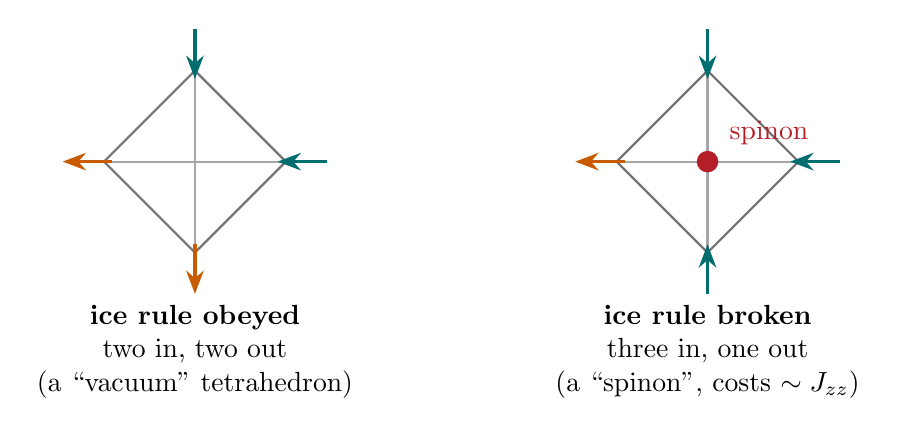
\begin{tikzpicture}[scale=1.05,>=Stealth]
% ---- left: ice rule obeyed ----
\begin{scope}
\coordinate (A) at (0,1.1); \coordinate (B) at (1.1,0);
\coordinate (C) at (0,-1.1); \coordinate (D) at (-1.1,0);
\draw[thick,black!55] (A)--(B)--(C)--(D)--cycle;
\draw[thick,black!35] (A)--(C); \draw[thick,black!35] (B)--(D);
% two in (A,B), two out (C,D)
\draw[->,very thick,icecol] (0,1.6)--(0,1.0);
\draw[->,very thick,icecol] (1.6,0)--(1.0,0);
\draw[->,very thick,spincol] (0,-1.0)--(0,-1.6);
\draw[->,very thick,spincol] (-1.0,0)--(-1.6,0);
\node[align=center] at (0,-2.3) {\textbf{ice rule obeyed}\\ two in, two out\\ (a ``vacuum'' tetrahedron)};
\end{scope}
% ---- right: defect ----
\begin{scope}[xshift=6.2cm]
\coordinate (A) at (0,1.1); \coordinate (B) at (1.1,0);
\coordinate (C) at (0,-1.1); \coordinate (D) at (-1.1,0);
\draw[thick,black!55] (A)--(B)--(C)--(D)--cycle;
\draw[thick,black!35] (A)--(C); \draw[thick,black!35] (B)--(D);
% three in, one out
\draw[->,very thick,icecol] (0,1.6)--(0,1.0);
\draw[->,very thick,icecol] (1.6,0)--(1.0,0);
\draw[->,very thick,icecol] (0,-1.6)--(0,-1.0);
\draw[->,very thick,spincol] (-1.0,0)--(-1.6,0);
\fill[badcol] (0,0) circle (0.13);
\node[badcol,right] at (0.15,0.35) {spinon};
\node[align=center] at (0,-2.3) {\textbf{ice rule broken}\\ three in, one out\\ (a ``spinon'', costs $\sim\Jzz$)};
\end{scope}
\end{tikzpicture}
\caption{One tetrahedron of the pyrochlore lattice, seen from above.  Each of
the four corners carries a spin that points in (teal) or out (orange).
Left: an ice-rule configuration.  Right: flipping one spin creates a defect
--- a \emph{spinon} --- with an energy cost of order $\Jzz$.}
\label{fig:icerule}
\end{figure}

The ice rule does not pick a single winner.  On a lattice of $N$ spins there
is an enormous number of different arrangements that all satisfy ``two in,
two out'' on every tetrahedron --- for our 16-site simulation cell there are
exactly 90 of them, for the 32-site cell 2970.  This collection of equally
happy states is called the \textbf{ice manifold}.  All the interesting
low-temperature physics happens \emph{inside} this collection.

\subsection{Three characters emerge}

Quantum mechanics lets the system tunnel between different ice configurations,
and out of this tunneling emerges a spectacular fiction: the system behaves,
at low energy, like a miniature universe with its own electromagnetism.
Three characters matter for us:

\begin{description}
\item[Spinons.] Break the ice rule on one tetrahedron (three-in--one-out)
and you create a particle-like defect.  Spinons are the ``electric charges''
of the emergent electromagnetism.  They are expensive (energy $\sim\Jzz$) and
show up in measurements as a broad feature at temperatures $T\sim\Jzz/4$.

\item[The photon / ring exchange.]  Within the ice manifold, the cheapest
quantum motion is a \emph{ring exchange}: six spins arranged around a
hexagonal loop flip together (in$\to$out$\to$in$\cdots$ becomes
out$\to$in$\to$out$\cdots$).  This collective six-spin flip is the matrix
out of which the emergent ``light'' (the photon) is built.  Its strength is
tiny:
\begin{equation}
\gsix \;=\; \frac{12\,|\Jpm|^{3}}{\Jzz^{2}},
\label{eq:g6}
\end{equation}
where $\Jpm$ is the quantum (spin-flipping) part of the interaction.  The
power \emph{three} appears because the loop must be built in three elementary
steps (more on this below).

\item[Flux.]  Going around a hexagon, the quantum amplitudes can add up as if
a magnetic flux threads the loop.  For $\Jpm<0$ (the sign relevant to the
cerium materials) theory predicts \emph{$\pi$-flux}: each hexagon behaves as
if half a flux quantum pierces it.  Detecting this flux is one of the big
experimental goals.
\end{description}

\begin{plainwords}
A magnet whose spins obey an ice rule hides a fictional universe: defects act
like electric charges (spinons), collective six-spin flips act like light
(photons), and hexagons can carry magnetic flux.  The photon scale $\gsix$ is
minuscule --- it involves $|\Jpm|^3$, the cube of an already small number ---
so any pollution of the simulation at a \emph{lower} power of $\Jpm$ will
drown it.  Keep that sentence in mind; it is the whole story.
\end{plainwords}

\subsection{The Hamiltonian, for reference}

For completeness (skip freely), the model is the XXZ pyrochlore Hamiltonian
\begin{equation}
H \;=\; \Jzz \sum_{\langle ij\rangle} S^{z}_i S^{z}_j
\;-\; \Jpm \sum_{\langle ij\rangle}\bigl(S^{+}_i S^{-}_j + S^{-}_i S^{+}_j\bigr),
\label{eq:H}
\end{equation}
with $\Jzz>0$ fixed to $1$ (it just sets the unit of energy) and the single
dial $\Jpm$, typically a few percent of $\Jzz$ in real materials, negative for
the cerium pyrochlores.  $S^z$ is the in/out arrow; $S^{\pm}$ flips it.

%=====================================================================
\section{The instrument: exact diagonalization on a torus}

\subsection{Why small boxes}

``Exact diagonalization'' (ED) means: write down \emph{every} possible spin
configuration, build the full table of quantum amplitudes between them, and
let the computer find the exact energy levels.  No approximation whatsoever
--- that is its glory.  Its curse is size: with $N$ spins there are $2^N$
configurations.  Sixteen spins give 65\,536 states (easy); 32 spins give 4.3
billion (heroic); 48 spins is beyond any computer for the full problem.  So
ED lives in small boxes, and to avoid fake surfaces we wrap the box around:
the right edge is glued to the left edge, the top to the bottom, front to
back.  A box glued this way is a \textbf{torus} --- a doughnut (in three
dimensions, a triple doughnut).

\subsection{Two kinds of loops on a doughnut}

On a doughnut there are two fundamentally different kinds of closed loops,
and this distinction is the geometric heart of the entire campaign.

\begin{figure}[h]
\centering
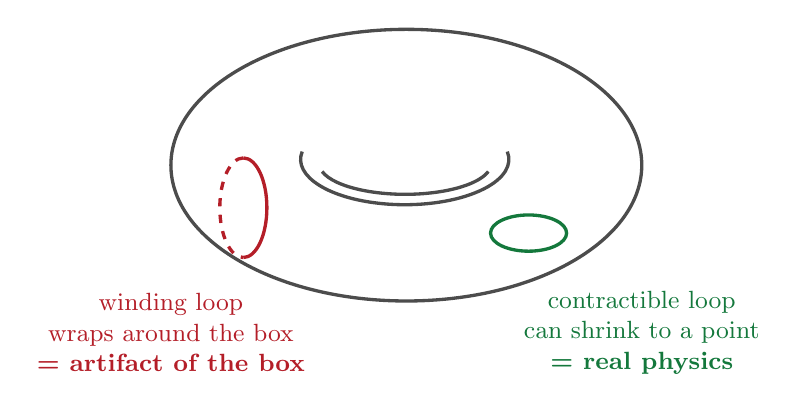
\begin{tikzpicture}[scale=1.15]
% torus
\draw[very thick,black!70] (0,0) ellipse (2.6 and 1.5);
\draw[very thick,black!70] (-1.15,0.15) arc (170:370:1.15 and 0.5);
\draw[very thick,black!70] (-0.93,-0.07) arc (195:345:0.95 and 0.34);
% contractible loop
\draw[goodcol,very thick] (1.35,-0.75) ellipse (0.42 and 0.2);
\node[goodcol,align=center,font=\small] at (2.6,-1.85) {contractible loop\\ can shrink to a point\\ \textbf{= real physics}};
% winding loop around the tube
\draw[badcol,very thick] (-1.8,-1.02) arc (-90:90:0.26 and 0.55);
\draw[badcol,very thick,dashed] (-1.8,0.08) arc (90:270:0.26 and 0.55);
\node[badcol,align=center,font=\small] at (-2.6,-1.85) {winding loop\\ wraps around the box\\ \textbf{= artifact of the box}};
\end{tikzpicture}
\caption{On a torus (a box with glued edges) a loop either shrinks to a point
(green) or wraps around the box and cannot shrink (red).  In an infinite
crystal only the first kind exists.  Everything the box invents lives on the
second kind.}
\label{fig:torus}
\end{figure}

\begin{description}
\item[Contractible loops] can be shrunk continuously to a point without ever
leaving the surface.  These loops exist in the infinite crystal too.  The
hexagonal ring exchange --- the photon --- lives on contractible loops.

\item[Winding loops] wrap around the doughnut.  They exist \emph{only
because the box has been glued shut}.  In the infinite crystal there is
nothing they correspond to.  Any process that lives on a winding loop is,
by construction, an artifact of the simulation geometry.
\end{description}

The number of times a loop wraps around each of the three glued directions is
called its \textbf{winding} $w=(w_x,w_y,w_z)$, three whole numbers.
Contractible loops have $w=(0,0,0)$.  A deep mathematical fact (we will meet
it again in Section~\ref{sec:mask}) says this triple of integers is the
\emph{only} topological label a loop on a torus carries --- there is no finer
distinction.

%=====================================================================
\section{The villain: the box invents a process stronger than the physics}
\label{sec:villain}

\subsection{Counting steps}

How strong is a collective flip process?  In quantum mechanics, a process
that requires $k$ elementary spin flips, each of strength $\Jpm$, passing
through intermediate states that cost energy $\sim\Jzz$, has strength roughly
\[
\frac{(\text{flip strength})^{k}}{(\text{energy barrier})^{k-1}}
\;=\;\frac{|\Jpm|^{k}}{\Jzz^{\,k-1}} .
\]
Each flip is a ``step up the ladder'', and cheaper processes need fewer
steps.  The hexagon needs six spins flipped, done in three neutral steps
(each step flips a $+$/$-$ pair), giving the $|\Jpm|^3$ of
Eq.~\eqref{eq:g6}.

Here is the catastrophe.  On the small torus there exist closed loops of only
\emph{four} sites that respect the ice rule --- but every single one of them
\textbf{wraps around the box}.  (In the infinite pyrochlore lattice the
shortest ice-respecting loop is the hexagon; the four-site loop only closes
because the glued boundary gives it a shortcut.)  A four-site loop needs just
two neutral steps:
\begin{equation}
\gfour \;=\; \frac{4\,\Jpm^{2}}{\Jzz}.
\label{eq:g4}
\end{equation}

\begin{figure}[h]
\centering
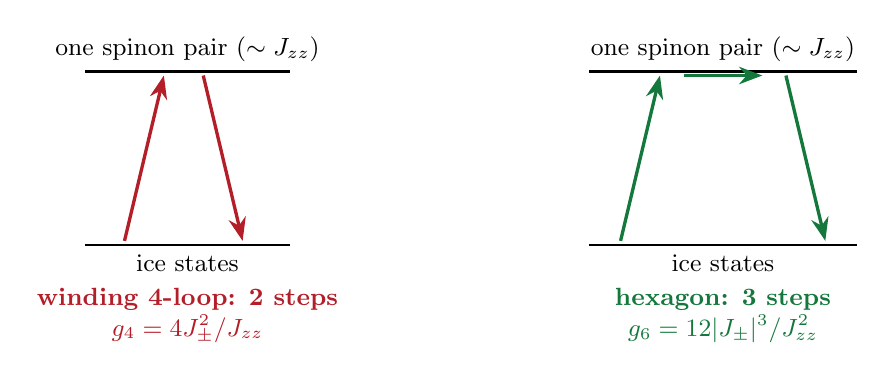
\begin{tikzpicture}[scale=1.0,>=Stealth]
% left: two-step ladder
\begin{scope}
\draw[thick] (0,0) -- (2.6,0); \node[below,font=\small] at (1.3,0) {ice states};
\draw[thick] (0,2.2) -- (2.6,2.2); \node[above,font=\small] at (1.3,2.2) {one spinon pair ($\sim\Jzz$)};
\draw[->,very thick,badcol] (0.5,0.05) -- (1.0,2.15);
\draw[->,very thick,badcol] (1.5,2.15) -- (2.0,0.05);
\node[badcol,align=center,font=\small] at (1.3,-0.9) {\textbf{winding 4-loop: 2 steps}\\ $\gfour = 4\Jpm^2/\Jzz$};
\end{scope}
% right: three-step ladder
\begin{scope}[xshift=6.4cm]
\draw[thick] (0,0) -- (3.4,0); \node[below,font=\small] at (1.7,0) {ice states};
\draw[thick] (0,2.2) -- (3.4,2.2); \node[above,font=\small] at (1.7,2.2) {one spinon pair ($\sim\Jzz$)};
\draw[->,very thick,goodcol] (0.4,0.05) -- (0.9,2.15);
\draw[->,very thick,goodcol] (1.2,2.15) -- (2.2,2.15);
\draw[->,very thick,goodcol] (2.5,2.15) -- (3.0,0.05);
\node[goodcol,align=center,font=\small] at (1.7,-0.9) {\textbf{hexagon: 3 steps}\\ $\gsix = 12|\Jpm|^3/\Jzz^2$};
\end{scope}
\end{tikzpicture}
\caption{Why the artifact beats the physics.  The fake wrap-around loop
completes in two steps, the genuine hexagon needs three.  Every extra step
costs one more factor of the small number $|\Jpm|/\Jzz$.}
\label{fig:ladder}
\end{figure}

The ratio of fake to real is
\begin{equation}
\frac{\gfour}{\gsix} \;=\; \frac{\Jzz}{3\,|\Jpm|},
\end{equation}
which \emph{grows} as the coupling gets smaller --- precisely in the
physically relevant regime.  At $\Jpm=-0.05$ the artifact is about seven
times stronger than the photon; at $\Jpm=-0.01$, thirty-three times.  And the
box is full of these loops: the 16-site cell hosts 36 winding four-site loops
and 48 boundary-wrapping hexagons, against only 16 genuine contractible
hexagons.

\subsection{The measured symptom}

The clearest thermodynamic fingerprint of the photon sector is a bump (a
``Schottky anomaly'') in the specific heat $C(T)$ at a temperature set by the
ring-exchange scale.  The campaign measured, across the whole coupling range,
where naive ED puts this bump:

\begin{center}
\begin{tabular}{lccc}
\toprule
 & peak follows & measured exponent & ideal exponent\\
\midrule
naive periodic ED & $\gfour$ \; ($T_{\rm peak}/\gfour \approx 1.9\to1.5$) & $|\Jpm|^{1.99}$ & 2 \\
winding-free ED & $\gsix$ \; ($T_{\rm peak}/\gsix \to 1.02$ as $\Jpm\to0$) & $|\Jpm|^{3.10}$ & 3 \\
\bottomrule
\end{tabular}
\end{center}

Measured against the photon scale $\gsix$, the naive peak position wanders by
a factor of \emph{forty} across the scan.  Naive ED does not measure the ring
scale badly --- it does not measure it \emph{at all}; it measures the box.

\begin{plainwords}
The simulation box invents a two-step shortcut process that only exists
because the edges are glued together.  The real photon is a three-step
process.  Since every step costs a factor of a small number, the fake
two-step process dominates everything the simulation says about the photon:
the low-temperature specific-heat bump, the flux, the dynamics.  The fake even
gets the \emph{sign of the flux wrong}: the naive ground state shows
zero-flux-like behaviour ($\langle$hexagon$\rangle = +0.116$) for both signs of
$\Jpm$, where the true $\pi$-flux answer is negative.
\end{plainwords}

%=====================================================================
\section{First attempt: twist averaging --- and why it fails}
\label{sec:twist}

\subsection{The idea}

There is a classical trick for taming box effects, borrowed from electronic
structure theory: \emph{twisted boundary conditions}.  When a spin flip
crosses the glued edge, multiply its amplitude by a phase factor
$e^{i\theta}$ --- as if a magnetic flux $\theta$ were threaded through the
hole of the doughnut.  A process that wraps the box $w$ times picks up the
phase $w\,\theta$; a contractible process picks up nothing.  So, the hope
goes: \textbf{average over twists} and the wrapping processes, whose phases
rotate around the clock, cancel to zero, while the physics is untouched.

The campaign's original claim (June 2026) was exactly this.  \textbf{It is
wrong}, and understanding \emph{why} it is wrong was the first real
discovery.

\subsection{The failure, precisely}

A ring-exchange process is not one path --- it is the \emph{sum of two}
distinct virtual routes (which pair of spins flips first).  The twist phase
attaches to each \emph{route}, not to the loop as a whole:
\[
c(\theta) \;=\; -\frac{\gfour}{2}\Bigl(e^{-i N_A\cdot\theta} + e^{-i N_B\cdot\theta}\Bigr),
\qquad N_A + N_B = w .
\]
Only the \emph{sum} of the two route-phases equals the winding.  The
magnitude works out to $|c(\theta)| = \gfour\,|\cos(w\cdot\theta/2)|$ --- and
here is the trap: on the 16-site cell, \emph{every} winding four-loop has one
route that never crosses the glued edge at all ($N_A=0$, phase $1$).  Half of
the fake amplitude is twist-blind.

\begin{figure}[h]
\centering
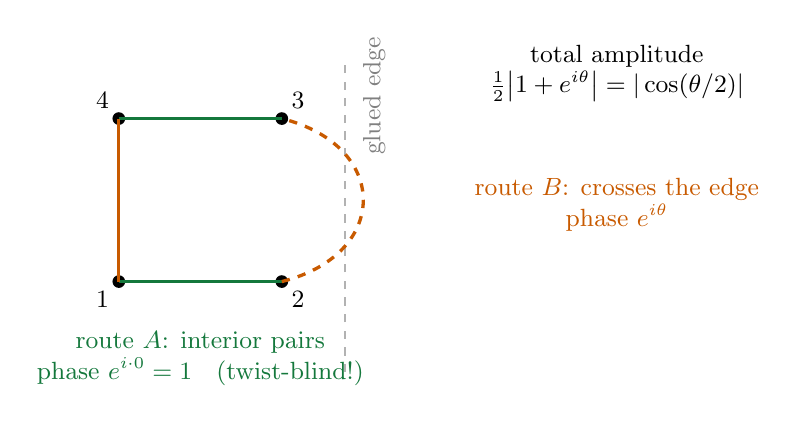
\begin{tikzpicture}[scale=1.15,>=Stealth]
% the winding square, 4 sites, boundary line
\draw[black!30,dashed,thick] (3.1,-0.7) -- (3.1,2.7);
\node[black!50,font=\small,rotate=90] at (3.42,2.35) {glued edge};
\fill (0.6,0.3) circle (0.07) node[below left,font=\small] {1};
\fill (2.4,0.3) circle (0.07) node[below right,font=\small] {2};
\fill (2.4,2.1) circle (0.07) node[above right,font=\small] {3};
\fill (0.6,2.1) circle (0.07) node[above left,font=\small] {4};
% route A: interior bonds (1,2) and (3,4)
\draw[goodcol,very thick] (0.6,0.3) -- (2.4,0.3);
\draw[goodcol,very thick] (2.4,2.1) -- (0.6,2.1);
\node[goodcol,font=\small,align=center] at (1.5,-0.55) {route $A$: interior pairs\\ phase $e^{i\cdot 0}=1$ \; (twist-blind!)};
% route B: bonds (2,3) via wrap and (4,1)
\draw[spincol,very thick,dashed] (2.4,0.3) .. controls (3.6,0.6) and (3.6,1.8) .. (2.4,2.1);
\draw[spincol,very thick] (0.6,2.1) -- (0.6,0.3);
\node[spincol,font=\small,align=center] at (6.1,1.15) {route $B$: crosses the edge\\ phase $e^{i\theta}$};
% resultant
\node[font=\small,align=center] at (6.1,2.6) {total amplitude\\ $\tfrac12\bigl|1+e^{i\theta}\bigr| = |\cos(\theta/2)|$};
\end{tikzpicture}
\caption{Why twist averaging cannot kill the wrap-around loop.  The four-spin
ring exchange is the sum of two virtual routes.  Route $B$ crosses the glued
edge and feels the twist; route $A$ uses only interior bonds and never sees
it.  No amount of averaging removes the twist-blind half.}
\label{fig:matchings}
\end{figure}

The campaign then quantified every version of the idea:
\begin{itemize}
\item \textbf{Averaging measured quantities} (compute $C(T)$ at each twist,
then average): weakest of all.  A measured quantity depends on the
\emph{square} of amplitudes, and squares of cosines never average to zero.
\item \textbf{Averaging over the special corner twists} $\theta\in\{0,\pi\}^3$:
keeps exactly half of every fake coupling.  Worse, a beautiful theorem
(Theorem~A below) shows these eight twists give \emph{identical} spectra ---
they are the same physics in eight disguises, so averaging them at the level
of observables does strictly nothing.
\item \textbf{The best possible single twist}, $\theta=(\pi/2,\pi/2,\pi/2)$:
kills 24 of the 36 fake loops exactly, but the other 12 survive at full
strength.  The surviving fraction of any twist-averaging scheme was proven to
have a hard floor of $1/3$ --- and because the surviving weight is
\emph{linear} in the choice of averaging weights, the optimum is a single
point: no clever ensemble beats the best single twist.
\item \textbf{The scaling test} (the damning one): with any observable-level
twist scheme, the specific-heat peak still scales as $|\Jpm|^{1.8}$ --- the
artifact power --- not the photon power $3$.  Twisting lowers the
contamination; it never changes what is being measured.
\end{itemize}

\begin{lesson}
The original ``theorem'' that twist averaging removes winding contamination
was retracted and the paper rewritten around the corrected theory.  Two
sub-lessons: (i) phases attach to virtual \emph{routes}, not to the loop's
topology --- always compute the object you claim vanishes; (ii) the special
twist $(\pi,\pi,\pi)$, which naively flips the sign of every wrapping bond,
was verified to leave the spectrum bit-for-bit unchanged --- it is a
\emph{gauge transformation}, a pure relabeling.  A sign flip of a matrix
element is not interference.
\end{lesson}

%=====================================================================
\section{The fix: a label that sees topology, and the mask}
\label{sec:mask}

\subsection{Transport: the bookkeeping number}

If phases cannot kill the winding loops, we must find something that
\emph{measures} winding exactly, and delete by hand.  The campaign found it,
and it is beautifully simple.

Every flip process moves magnetization around.  Take the set of spins the
process flips; add up their positions with a $+$ sign for raised spins and
$-$ for lowered ones.  This gives a vector $\rho$, the \textbf{transport} (or
polarization displacement) of the process.  The campaign proved, by explicit
enumeration over every loop of both simulation cells, the exact identity
\begin{equation}
\rho \;=\; \tfrac12\, w \cdot L,
\label{eq:rho}
\end{equation}
where $w$ is the winding and $L$ the box dimensions.  Read it aloud:
\emph{transport is half the winding}.  A contractible loop ($w=0$) transports
nothing --- the raised and lowered spins balance perfectly.  A winding loop
\emph{cannot} balance: it transports exactly half a box length.  There is no
overlap and no ambiguity: measuring $\rho$ \emph{is} measuring topology.

\subsection{The mask}

The recipe is now almost embarrassingly direct.  Group the 90 ice states into
families (``sectors'') that share the same value of the polarization; on the
16-site cell there are 25 such sectors.  Then, in the table of quantum
amplitudes between ice states:
\begin{center}
\emph{delete every entry that connects two different sectors.}
\end{center}
That is the whole method.  It is called the \textbf{mask}.  By
Eq.~\eqref{eq:rho}, an entry connecting different sectors is precisely a
process with $w\ne0$: a wrap-around artifact.  An entry within a sector is a
contractible process: untouched, to the last digit.

\begin{figure}[h]
\centering
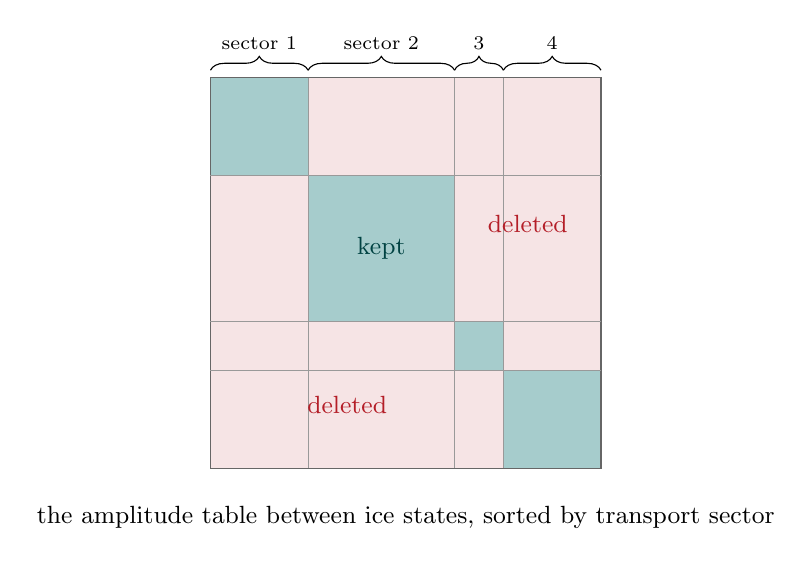
\begin{tikzpicture}[scale=0.62]
% 8x8 block matrix, blocks at 0-2,2-5,5-6,6-8
\fill[badcol!12] (0,0) rectangle (8,8);
\fill[icecol!35] (0,6) rectangle (2,8);
\fill[icecol!35] (2,3) rectangle (5,6);
\fill[icecol!35] (5,2) rectangle (6,3);
\fill[icecol!35] (6,0) rectangle (8,2);
\draw[black!60] (0,0) rectangle (8,8);
\foreach \x in {2,5,6} \draw[black!40] (\x,0) -- (\x,8);
\foreach \y in {2,3,6} \draw[black!40] (0,\y) -- (8,\y);
\node[font=\small,icecol!60!black] at (3.5,4.5) {kept};
\node[font=\small,badcol] at (6.5,5.0) {deleted};
\node[font=\small,badcol] at (2.8,1.3) {deleted};
\draw[decorate,decoration={brace,amplitude=5pt}] (0,8.15) -- (2,8.15)
  node[midway,above=4pt,font=\scriptsize,align=center] {sector 1};
\draw[decorate,decoration={brace,amplitude=5pt}] (2,8.15) -- (5,8.15)
  node[midway,above=4pt,font=\scriptsize,align=center] {sector 2};
\draw[decorate,decoration={brace,amplitude=5pt}] (5,8.15) -- (6,8.15)
  node[midway,above=4pt,font=\scriptsize] {3};
\draw[decorate,decoration={brace,amplitude=5pt}] (6,8.15) -- (8,8.15)
  node[midway,above=4pt,font=\scriptsize] {4};
\node[font=\small,align=center] at (4,-1.0) {the amplitude table between ice states, sorted by transport sector};
\end{tikzpicture}
\caption{The mask.  Sort ice states by their polarization sector; keep the
diagonal blocks (contractible physics, green), delete everything off the
blocks (wrap-around artifacts, red).  Deleting can only remove processes ---
it can never invent new ones.}
\label{fig:mask}
\end{figure}

\subsection{What the mask never asks: configurations, not eigenstates}
\label{sec:configs}

A question that sounds central but that the mask never answers --- because
it never asks it --- is: \emph{which eigenstates of $H$ are the ice band?}

Ice-ness, in this method, is a property of \emph{configurations}, not of
energy levels.  A basis pattern either satisfies two-in--two-out on every
tetrahedron or it does not --- a yes/no check made pattern by pattern,
tetrahedron by tetrahedron, involving no diagonalization, no energy
threshold, and no coupling constant.  The same 90 patterns qualify at
$\Jpm=-0.03$ and at $\Jpm=-0.5$.  The sectors and the mask inherit this:
they are combinatorial objects, fixed before any physics is computed.

``Band'' identity is then an \emph{output label, never an input
classification}.  A winding-free band level is, by definition, a
self-consistent root of an ice-sector block (the machinery of
Secs.~\ref{sec:feshbach} and~\ref{sec:strong}), and it arrives stamped with
its sector because that is where it emerged.  Even when such a root sits
embedded inside the continuum (Sec.~\ref{sec:bic}), there is no ambiguity
about whether it is ``band'': it is a root of the ice-block map, full stop.

The contrast to draw is with the \emph{frames} of
Sec.~\ref{sec:strong} --- constructions that answered the question the
other way around, by hunting for the 90 most ice-\emph{like eigenstates}.
All of them die at strong coupling, and necessarily so: once bands mix,
eigenstate identity is genuinely undefined.  The mask survives because it
staked its definition on something that cannot mix: the spin patterns
themselves.  (At strong coupling the physical states behind the roots are
only $\sim25\%$ ice by weight --- the map does not care; the ice patterns
say where a state is \emph{anchored}, and the fold of
Sec.~\ref{sec:feshbach} supplies everything else about it, exactly.)

\subsection{Why this is safe, and why nothing finer exists}

Three properties make the mask trustworthy:

\begin{enumerate}
\item \textbf{It only removes.}  A projection deletes entries; it cannot
create a process that was not there.  So it cannot introduce new physics.
\item \textbf{It provably keeps the physics.}  Contractible loops have
$\rho=0$ exactly (verified on every hexagon of both cells) and their
amplitudes are untouched to machine precision.
\item \textbf{It is maximal.}  The torus's mathematics (its ``fundamental
group'' is $\mathbb{Z}^3$: loops are classified by three whole numbers, full
stop) guarantees that winding is the \emph{only} topological label.  A
process that winds $+1$ and then $-1$ (net zero) is topologically identical
to a contractible one and is \emph{correctly kept} --- its counterpart exists
in the infinite crystal too, as an ordinary, benign finite-size correction.
The mask removes everything a topological label can remove, and nothing more.
\end{enumerate}

\subsection{Three theorems, in plain words}
\label{sec:theorems}

Later, the twist story and the mask story were united by three exact theorems
(each verified to fifteen digits):

\begin{description}
\item[Theorem A (the eight disguises).]  The eight corner twists
$\theta\in\{0,\pi\}^3$ produce \emph{identical} energy spectra --- each is
the untwisted problem seen through a relabeling of states.  Practical payoff:
anything requiring ``all eight corners'' needs \emph{one} computer run.
\item[Theorem B (average $=$ mask).]  The sophisticated ``character
average'' over the eight corners --- the operator-level averaging done right
--- is \emph{exactly} the parity version of the mask.  Verified entry by
entry: zero mismatches out of 8100.  The fancy procedure and the simple
deletion are the same object, and the deletion is eight times cheaper.
\item[Theorem C (the general dictionary).]  Any twist whatsoever factorizes
into (a relabeling) $\times$ (a genuine flux).  This explains every entry of
the old ``twists keep half'' table and closes the subject: twists and masks
are one theory, and the mask is its strongest element.
\end{description}

One more exact selection rule fell out as a bonus: within the winding-free
world, the uniform magnetization response at zero wavevector vanishes
\emph{identically} (measured: $5\times10^{-30}$, versus $0.333$ for naive
ED).  Every bit of that signal in a naive simulation is artifact.

\begin{plainwords}
Count, for each quantum process, how far it shifts the magnetization pattern.
Wrap-around processes shift it by half a box; real processes shift it by
zero.  Delete the shifters.  That single sentence is the method, it costs
almost nothing, it provably deletes all of the artifact and none of the
physics, and mathematics guarantees nothing sharper is possible.
\end{plainwords}

%=====================================================================
\section{A toolkit interlude: folding the universe into a small matrix}
\label{sec:feshbach}

Everything so far treated the ice manifold perturbatively --- valid when
$|\Jpm|$ is small.  The campaign's second act pushes into \emph{strong}
coupling, and for that we need one more tool, the \textbf{Feshbach map}
(also called a Schur complement).  Despite the name it is one idea:

\begin{quote}
\emph{You care about a few states (the 90 ice states, call them $P$).  The
other 12\,780 states (the spinon states, call them $Q$) matter only as
temporary stopovers.  Fold their effect into a corrected amplitude table for
the 90, and solve the small problem.}
\end{quote}

The folded table is
\begin{equation}
F(z) \;=\; \underbrace{PHP}_{\text{direct}} \;+\;
\underbrace{PHQ\,\frac{1}{z-QHQ}\,QHP}_{\text{out to }Q\text{ and back}},
\label{eq:feshbach}
\end{equation}
where $z$ is the energy at which you ask the question.  The exact energies of
the full problem below the spinon continuum are precisely the
self-consistent solutions of $E = \mathrm{eig}\,F(E)$: the answer feeds back
into the question.  Nothing is approximated --- $F$ at the right $z$
reproduces exact eigenvalues of the full $H$ to machine precision.

\begin{figure}[h]
\centering
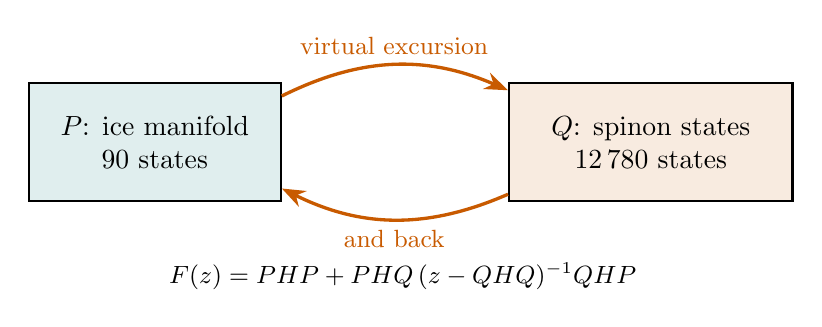
\begin{tikzpicture}[>=Stealth]
\node[draw,thick,fill=icecol!12,minimum width=3.2cm,minimum height=1.5cm,align=center]
  (P) at (0,0) {$P$: ice manifold\\ 90 states};
\node[draw,thick,fill=spincol!12,minimum width=3.6cm,minimum height=1.5cm,align=center]
  (Q) at (6.3,0) {$Q$: spinon states\\ 12\,780 states};
\draw[->,very thick,spincol] (P.20) to[bend left=25] node[above,font=\small]{virtual excursion} (Q.160);
\draw[->,very thick,spincol] (Q.200) to[bend left=25] node[below,font=\small]{and back} (P.-20);
\node[font=\small,align=center] at (3.15,-1.7)
  {$F(z) = PHP + PHQ\,(z-QHQ)^{-1}QHP$};
\end{tikzpicture}
\caption{The Feshbach idea: excursions into the huge spinon space are summed
exactly into a corrected $90\times90$ table.  No frames, no overlaps, no
approximation --- and it exists at \emph{any} coupling strength.}
\label{fig:feshbach}
\end{figure}

Two more characters:
\begin{description}
\item[$Z$, the \textbf{ice weight} (also: residue, purity).]  The fraction
of a state that actually lives in $P$.  It is a property of each exact
eigenstate $|n\rangle$ of the full $H$, not of the map:
\[
Z_n \;=\; \langle n|P|n\rangle \;=\; \bigl\| P|n\rangle \bigr\|^2
       \;=\!\!\!\!\sum_{c\,\in\,\text{two-in--two-out}}\!\!\!\!
         |\langle c|n\rangle|^2
       \;\in\;[0,1].
\]
Be precise about what is being projected onto.  The sum runs over the $90$
\emph{ice configurations} $|c\rangle$ --- the spin patterns obeying the ice
rule on every tetrahedron --- not over Ising configurations in general:
those form a complete basis, so projecting onto all of them is the identity
and every $Z_n$ would be $1$.  $P$ is the rank-90 projector onto the span
of that \emph{subset},
$P=\sum_{c\,\in\,\text{two-in--two-out}}|c\rangle\langle c|$, diagonal in
the Ising basis and purely combinatorial (Sec.~\ref{sec:configs}); its
complement $Q$ is spanned by the other $12\,780$ configurations, each of
which has at least one tetrahedron violating the rule, i.e.\ at least one
spinon pair.  So $Z_n$ is the total probability that a measurement in the
Ising basis returns an ice-obeying pattern.  $Z_n=1$ is a pure ice state,
$Z_n=0$ a state with no ice
content at all, and $1-Z_n$ is the \emph{spinon dressing}: the weight the
state has borrowed from $Q$ by breaking ice rules virtually.  One corollary
worth flagging early: because the ice manifold is a set of configurations
in the \emph{local-$z$} frame, $Z$ is defined relative to that frame ---
the same physical state has a different ice weight with respect to an
$x$-basis ice manifold.  Far from the Heisenberg point this is harmless
(the $z$ frame is the physical one); at it, it is the whole story
(Sec.~\ref{sec:heisenberg}).

Two properties make $Z$ more than a diagnostic.  First, it is obtainable
\emph{without} eigenvectors: at a self-consistent root $E_n$ of the
branch $\lambda_n(z)$ of $F(z)$, $Z_n=[1-\lambda_n'(E_n)]^{-1}$ --- the
flatter the folded map at a root, the purer the state (steep slope means
the answer depended strongly on the asking-energy, i.e.\ on the
excursions into $Q$).  Second, it obeys an exact sum rule,
$\sum_n Z_n = \mathrm{Tr}\,P = 90$, the sum running over \emph{all}
$12\,870$ eigenstates: the ice manifold's 90 dimensions are shared out
among the whole spectrum, and the shares always total 90.
Sec.~\ref{sec:twoside} turns that sum rule into a thermodynamic identity.
At weak coupling $Z\approx0.99$ (states are
almost pure ice); by $\Jpm=-0.30$, $Z\approx0.25$ --- states are mostly
spinon dressing.  $1-Z$ controls every error and every convergence rate in
what follows.
\item[The mask, again.]  The transport label is defined on ice states, so
the mask applies to $F(z)$ verbatim: delete entries of $F$ between different
sectors.  This ``masked Feshbach map'' is the campaign's precision
instrument: \emph{winding-free and valid at any coupling}.
\end{description}

\begin{worked}
A three-level miniature contains the whole method.  Take states
$|1\rangle,|2\rangle$ (our ``ice states'', in \emph{different} transport
sectors) and $|3\rangle$ (the ``spinon''), with flip strength $t=0.2$ into
$|3\rangle$ and spinon cost $D=1$:
\[
H=\begin{pmatrix}0&0&t\\ 0&0&t\\ t&t&D\end{pmatrix}.
\]
\textbf{Fold:} excursions $1\to3\to2$ give
$F(z)=\begin{pmatrix}f&f\\ f&f\end{pmatrix}$ with $f=-t^2/(D-z)$.
The \emph{off-diagonal} $f$ connects different sectors: it is the analogue of
a winding amplitude, generated purely by passing through the spinon.
\textbf{Solve self-consistently:} $z=2f(z)$ gives
$z_0=\tfrac12\bigl(D-\sqrt{D^2+8t^2}\bigr)=-0.074456$, which is exactly the
ground state of the full $3\times3$ matrix --- fold-and-solve is exact.
\textbf{Mask:} delete the off-diagonal; each sector alone solves
$z=f(z)$, giving $z=\tfrac12\bigl(1-\sqrt{1.16}\bigr)=-0.038517$, twice
(exactly degenerate) --- the winding-free answer.  Note it is roughly
\emph{half} the raw binding: on the real cluster, too, about half of the
naive ground-state depth is artifact.
\textbf{Counterterm} (Section~\ref{sec:hc}): add $+0.037228$ to cancel the
off-diagonal at $z_0$; the resulting honest Hamiltonian gives levels
$-0.039716$ and $-0.037228$ --- centred on the exact $-0.038517$ but split
by $0.0025$.  That split is the ``residual $z$-dependence'': the counterterm
cancels the artifact perfectly at one energy and imperfectly nearby.  The
purity here is $Z=0.9352$; the split grows as $1-Z$.  Every phenomenon of
the real campaign appears in this $3\times3$ example.
\end{worked}

%=====================================================================
\section{Strong coupling: the band dissolves, and the map survives}
\label{sec:strong}

\subsection{What breaks, and when}

As $|\Jpm|$ grows, the neat separation ``cheap ice band far below expensive
spinons'' degrades.  On the 16-site cell the ice-derived band stops being
cleanly separated from the two-spinon continuum at $\Jpm\approx-0.185$.
Every earlier construction that relied on identifying ``the 90 ice-like
eigenstates'' (so-called frames) fails there --- and the campaign showed all
of them fail \emph{together}, because every one of their health diagnostics
secretly measures the same quantity: the ice purity $Z$.  There is no
cleverer frame; the concept of ``pick the ice-like eigenvectors'' itself
runs out.

\begin{figure}[h]
\centering
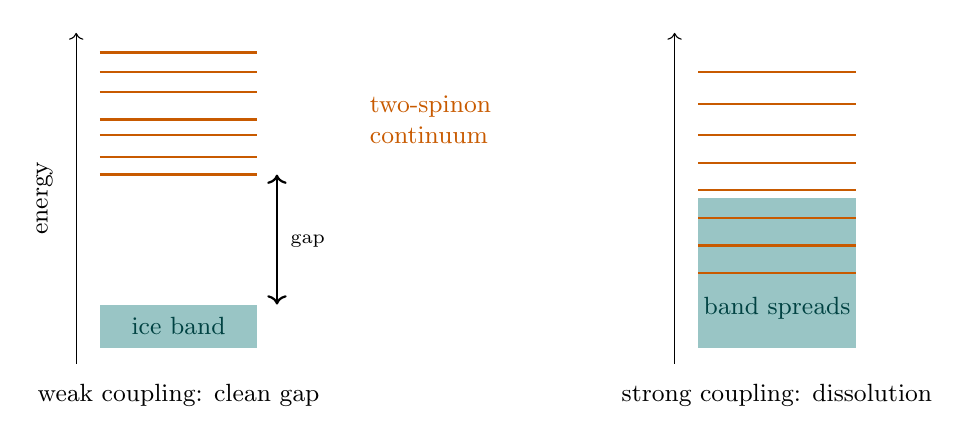
\begin{tikzpicture}[scale=1.0]
% left panel: weak coupling
\begin{scope}
\draw[->] (0,0) -- (0,4.2); \node[rotate=90,font=\small] at (-0.4,2.1) {energy};
\fill[icecol!40] (0.3,0.2) rectangle (2.3,0.75);
\node[font=\small,icecol!60!black] at (1.3,0.475) {ice band};
\foreach \y in {2.4,2.62,2.9,3.1,3.45,3.7,3.95} \draw[spincol,thick] (0.3,\y) -- (2.3,\y);
\node[font=\small,spincol] at (1.3,4.05) {\vphantom{g}};
\node[font=\small,spincol] at (1.35,2.15) {\vphantom{g}};
\node[font=\small,spincol,above] at (1.3,3.95) {};
\node[font=\small] at (1.3,-0.4) {weak coupling: clean gap};
\draw[<->,thick] (2.55,0.75) -- (2.55,2.4);
\node[font=\scriptsize,right] at (2.6,1.55) {gap};
\node[font=\small,spincol] at (1.3,3.3) {};
\node[font=\small,spincol,align=center] at (1.3,1.6) {};
\node[font=\scriptsize,spincol] at (1.3,2.62) {};
\node[font=\scriptsize,spincol,above right] at (0.3,2.9) {};
\node[font=\small,spincol] at (3.9,3.2) {};
\end{scope}
\node[font=\small,spincol,align=left] at (4.5,3.1) {two-spinon\\ continuum};
% right panel: strong coupling
\begin{scope}[xshift=7.6cm]
\draw[->] (0,0) -- (0,4.2);
\fill[icecol!40] (0.3,0.2) rectangle (2.3,2.1);
\node[font=\small,icecol!60!black,align=center] at (1.3,0.7) {band spreads};
\foreach \y in {1.15,1.5,1.85,2.2,2.55,2.9,3.3,3.7} \draw[spincol,thick] (0.3,\y) -- (2.3,\y);
\node[font=\small] at (1.3,-0.4) {strong coupling: dissolution};
\end{scope}
\end{tikzpicture}
\caption{Weak coupling (left): the ice-derived band sits far below the
spinon continuum.  Strong coupling (right): the band widens and the continuum
descends until they interpenetrate.  Constructions that must \emph{identify}
band states die here; the Feshbach map, which never identifies anything, does
not.}
\label{fig:dissolve}
\end{figure}

\subsection{What survives}

The masked Feshbach map does not care: it is built from the ice
\emph{configurations} (which exist at any coupling --- they are just spin
patterns), not from eigenvectors.  Its self-consistent roots below the
continuum edge remain exact, winding-free energies at every coupling tested.
Highlights of the strong-coupling reconnaissance on the 16-site cell:

\begin{itemize}
\item \textbf{Completeness:} all 90 winding-free levels exist below the
continuum up to $\Jpm=-0.22$; at $-0.24$ to $-0.26$ one goes missing; at
$-0.28$, thirteen (77 of 90 remain).  The missing ones did not die --- see
next item.
\item \textbf{The escaped levels are not lost.}  They reappear \emph{above}
the continuum edge with exactly zero decay width, still tracked cleanly by
the masked map.  How that is possible --- and when it stops being possible
--- deserves its own subsection (Sec.~\ref{sec:bic}).
\item \textbf{The flux law is restored.}  The naive ground state gets the
sign of the hexagon flux wrong at every coupling; the winding-free ground
multiplet gives the correct $\pi$-flux sign throughout, fading smoothly as
coupling grows ($\langle\text{hex}\rangle = -0.248$ at $-0.02$ down to
$-0.067$ at $-0.30$).
\item \textbf{Nothing dramatic happens to the raw ground state:} it evolves
smoothly to $\Jpm=-1$ with no level crossing.  The drama --- band
dissolution --- is real physics of the \emph{excitations}, and it is
continuous, not a wall.  (Its interpretation as a Higgs-type frontier of the
emergent gauge theory is a separate, ongoing project.)
\end{itemize}

\subsection{Life inside the continuum: tracking without repairing}
\label{sec:bic}

What does it actually mean for a gauge-band level to ``enter the spinon
continuum''?  The masked map answers this with unusual precision, because it
is not one map but twenty-five: one independent block per transport sector,
and \emph{each block has its own continuum} --- the spinon states that
particular sector can reach.  The global ``continuum edge'' quoted in
dissolution plots is just the lowest of these.

So when a level of sector $A$ rises above the \emph{global} edge, the first
question is: whose continuum is it swimming in?  If the spinon states at
that energy connect to \emph{other} sectors, the level of sector $A$ cannot
decay into them --- the transport label forbids it --- and sector $A$'s own
map still has a perfectly ordinary, real, self-consistent root there.  The
level is a \textbf{bound state in the continuum} (BIC): embedded in the
spectrum, yet with decay width exactly zero.  This is not a hope but a
measurement: the multiplets that escaped the band at strong coupling were
recovered this way (for example a twelve-fold multiplet sitting $0.16\,\Jzz$
\emph{above} the edge, width zero to machine precision).  This is why the
winding-free photon never decays in the regime we mapped, and why the
``band merging'' seen in naive ED there is frame artifact rather than a
physical lifetime.

\begin{figure}[h]
\centering
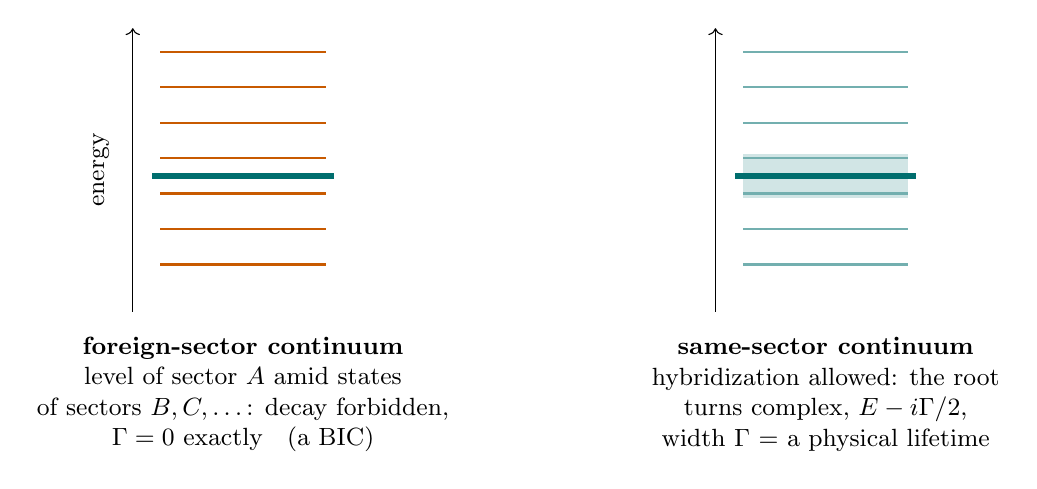
\begin{tikzpicture}[scale=1.0]
% left: BIC
\begin{scope}
\draw[->] (0,0) -- (0,3.6);
\node[rotate=90,font=\small] at (-0.4,1.8) {energy};
\foreach \y in {0.6,1.05,1.5,1.95,2.4,2.85,3.3}
  \draw[spincol,thick] (0.35,\y) -- (2.45,\y);
\draw[icecol,line width=2.2pt] (0.25,1.72) -- (2.55,1.72);
\node[font=\small,align=center] at (1.4,-1.05)
  {\textbf{foreign-sector continuum}\\ level of sector $A$ amid states\\
   of sectors $B,C,\dots$: decay forbidden,\\ $\Gamma=0$ exactly \; (a BIC)};
\end{scope}
% right: resonance
\begin{scope}[xshift=7.4cm]
\draw[->] (0,0) -- (0,3.6);
\fill[icecol!18] (0.35,1.45) rectangle (2.45,2.0);
\foreach \y in {0.6,1.05,1.5,1.95,2.4,2.85,3.3}
  \draw[icecol!55,thick] (0.35,\y) -- (2.45,\y);
\draw[icecol,line width=2.2pt] (0.25,1.72) -- (2.55,1.72);
\node[font=\small,align=center] at (1.4,-1.05)
  {\textbf{same-sector continuum}\\ hybridization allowed: the root\\
   turns complex, $E-i\Gamma/2$,\\ width $\Gamma$ = a physical lifetime};
\end{scope}
\end{tikzpicture}
\caption{Two very different ways to sit inside a continuum.  Left: the
surrounding continuum belongs to other transport sectors (orange); the
masked map's per-sector root stays real and the state cannot decay --- the
mask keeps tracking it effortlessly.  Right: the continuum in the state's
\emph{own} sector has reached it; the real root disappears and the honest
object is a complex ``Gamow'' root whose imaginary part is a genuine decay
rate --- physics to be reported, not an artifact to be repaired.}
\label{fig:bic}
\end{figure}

The mechanism has a genuine failure mode, and it is the physically
interesting one.  When the continuum \emph{in the state's own sector}
reaches the level, nothing forbids hybridization: the real self-consistent
root ceases to exist, and the correct object becomes a complex root
$E - i\Gamma/2$ (a ``Gamow'' resonance).  At that point the width $\Gamma$
is not an error to be subtracted --- it is a prediction: a finite photon
lifetime, if the infinite system truly has one, must be allowed to appear
exactly here.  The mask has not lost track of the state; it has changed
\emph{what kind of object it reports}, from a level to a resonance.

Two honesty caveats keep this from being too tidy:
\begin{itemize}
\item On a finite cluster the ``continuum'' is itself a handful of discrete
levels, so same-sector contact shows up as avoided crossings: the band
state's identity smears over several eigenstates, and tracking it becomes a
matter of following \emph{spectral weight}, not a single number.
\item Whether a level is inside or outside the continuum depends on where
the edge sits --- and on a small cluster the edge is one of the
\emph{worst}-converged quantities there is.  A verdict of ``escaped'' can be
an artifact of a misplaced edge.  This is precisely the itch that the
continuum-densification pillar of the next campaign
(Sec.~\ref{sec:roadahead}) scratches.
\end{itemize}

\begin{lesson}
\textbf{The unconverged fixed point.}  Solving $E=\mathrm{eig}\,F(E)$ by
simple repetition (guess $E$, compute, feed back) converges at rate $1-Z$
per round.  At strong coupling $1-Z\approx0.5$, so three rounds leave a
residual of about $10^{-2}$ --- which was, for one embarrassing week,
misread as a new physical effect (an ``anchoring residue'', complete with a
spurious extra peak in $C(T)$).  A proper root-finder (a secant step)
reaches $10^{-13}$ in 5--11 solves, and the ``effect'' evaporated: the
ground multiplet is degenerate to $10^{-12}$, the spurious peak gone.
Moral: before interpreting a small number as physics, converge it.
\end{lesson}

\begin{lesson}
\textbf{The physical third peak.}  After the spurious peak was removed, a
\emph{different} extra bump in $C(T)$ at $|\Jpm|\ge0.22$ survived every
convergence test --- because it is real: a Schottky anomaly from a genuine
gap inside the winding-free spectrum.  At weak coupling it coincides with
the ring bump and hides; at strong coupling they separate.  One artifact
peak and one physical peak had been conflated.  Moral: not every surprise is
a bug; the same rigor that kills artifacts must be allowed to certify
physics.  (The story goes deeper: ``the third peak'' turned out to name
\emph{three} distinct low-temperature bumps --- one fake, two real.  The
full taxonomy, separated cleanly by the fold data, is
Sec.~\ref{sec:thirdpeak}.)
\end{lesson}

%=====================================================================
\section{One honest Hamiltonian: the counterterm, its limits, the splice}
\label{sec:hc}

\subsection{Why there is nothing to cut: the ice block of $H$ is empty}
\label{sec:emptyblock}

The masked map is exact but speaks only about the ice-derived band.  For
full thermodynamics --- both peaks of $C(T)$, entropy, flux on the true
dressed ground state --- one wants a single honest Hamiltonian on the
\emph{whole} space.  The natural first idea is pure surgery: take the full
$H$, find the winding matrix elements between ice states, delete them, and
leave everything else connected.  No counterterm, no anchor --- just a
scalpel.

This fails for a startling reason: \textbf{there are no such matrix
elements}.  The ice block of the bare Hamiltonian, $PHP$, is
\emph{diagonal}.  A single pair-flip acting on an ice state always breaks
the ice rule on the tetrahedra it touches --- it necessarily creates
spinons and lands in $Q$.  No ice state connects to any other ice state
directly.  Both the physical hexagon amplitude $\gsix$ \emph{and} the
winding artifact $\gfour$ are emergent: assembled from multi-step paths
that leave the ice manifold, wander through spinon space, and return.
They live inside the resolvent $(z-QHQ)^{-1}$, smeared across the
geometry of $Q$ --- not in any entry of $H$ a scalpel could reach.  The
$3\times3$ miniature of Sec.~\ref{sec:feshbach} shows it nakedly: the
offending amplitude is $-t^2/(D-z)$, and no entry of the original matrix
contains it; the matrix holds only $t$ and $D$.

This is why deletion (the mask) operates on $F(z)$ --- where the emergent
amplitudes have \emph{become} explicit matrix elements --- and can never be
performed on $H$ itself.  On $H$, the only possible surgery is
\textbf{addition}: insert a new ice-block operator whose emergent effect
cancels the winding paths.  The counterterm is not a clever choice among
alternatives; it is the only move the structure of $H$ permits.  And note
that the ``reconnection to the full Hamiltonian'' comes free: the added
operator touches only the $90\times90$ ice block, while $PHQ$, $QHP$, and
$QHQ$ remain byte-for-byte intact --- spinons, dressing, and the upper
band still flow through the untouched couplings.

\subsection{The construction}

The campaign's construction, forced by the above: compute the masked-out
(artifact) part of $F$ at the self-consistent ground energy $z_0$, and
\emph{subtract it from $H$} as a counterterm $C$ supported purely inside the
ice block:
\[
H + C, \qquad C = -(1-\Delta)\,F(z_0)
\quad (\Delta = \text{the mask}).
\]
Because $C$ lives inside the ice block, it does not disturb the spinon
sector at all, and one ordinary diagonalization of $H+C$ delivers the entire
65\,536-level spectrum, winding-free through third order in every loop class
at once.  This is the object behind the money plot of the campaign
(the specific-heat scan of Section~\ref{sec:results}).

\subsection{The obstruction theorem, and honesty about the residue}

Can the counterterm be made \emph{exactly} winding-free at all energies?
\textbf{No --- provably.}  The transport label is only defined on ice
states; a single spinon hop moves the polarization by a quarter of a box
period, so no rule on the full space can conserve the label.  Consequently
$H+C$ carries an irreducible residual error that grows with the dressing:
about $0.4\%$ of the bandwidth at $\Jpm=-0.02$, $7\%$ at $-0.10$, $22\%$ at
$-0.30$ --- the $3\times3$ miniature's level split, writ large.  The
division of labor is therefore:

\begin{center}
\begin{tabular}{lll}
\toprule
question & instrument & why\\
\midrule
band energies, ring scale, flux & masked Feshbach roots & exact at any coupling\\
full $C(T)$, entropy, upper peak & $H+C$ spectrum & only full-space object\\
best of both & \textbf{the splice} & see below\\
\bottomrule
\end{tabular}
\end{center}

\textbf{The splice} replaces the lowest 90 levels of the $H+C$ spectrum by
the exact masked roots.  Wherever the band is complete
($|\Jpm|\lesssim0.22$ on 16 sites) the result is clean: exactly two peaks in
$C(T)$, correct scales, no artifact.

\subsection{What the counterterm cannot do}
\label{sec:hclimits}

A natural hope: when band levels escape into the continuum
(Sec.~\ref{sec:bic}), perhaps $H+C$ ``replaces'' them too, carrying the
correction into the dissolution regime.  It does not --- doubly, and
provably.

First, $C$ is \textbf{static and anchored}: it is built from $F$ evaluated
at one energy, the ground-state anchor $z_0$.  The states that run into the
continuum are precisely the ones \emph{farthest} from the anchor and the
most spinon-dressed --- so the cancellation is at its \emph{worst} exactly
for them.  That is the $1-Z$ residue of the previous subsection, seen from
the other side.

Second, \textbf{the splice cannot rescue them}.  The splice presumes a
one-to-one assignment between ``the lowest 90 levels of $H+C$'' and ``the
90 masked roots''.  Once band levels and continuum levels interleave, that
assignment simply does not exist: an escaped masked root sits \emph{among}
continuum eigenvalues of $H+C$, and there is no principled rule for which
one it replaces.  This --- not numerical difficulty --- is why the splice
is certified clean only up to $|\Jpm|\approx0.22$ on this cluster.

Nor can a smarter counterterm be built.  Making $C$ follow the escaped
states would require either an energy-\emph{dependent} $C(z)$ --- but then
$H+C$ is no longer a Hamiltonian and its thermodynamics is ill-defined ---
or a transport projection on the full space, which the obstruction theorem
of the previous subsection forbids exactly (the spinon hop moves the label
by a quarter period; no Hermitian operator conserves it).  The wall is
structural.

So in the dissolution regime the division of labor genuinely shifts: the
per-sector masked map --- with its BICs and Gamow widths --- is the
\emph{only} exact instrument for band physics, while $H+C$ degrades to a
gross thermodynamic estimate whose growing residue must be quoted alongside
it.  Whether one can do better --- dropping the counterterm altogether ---
is the subject of the next subsection.

\subsection{A counterterm-free future: folding from both sides}
\label{sec:twoside}

The Feshbach fold of Sec.~\ref{sec:feshbach} has a mirror image.  Just as
$F(z)$ folds the spinon space into a corrected ice-block table, one can
fold the ice space into a corrected \emph{spinon}-block table:
\[
G(z) \;=\; QHQ \;+\; QHP\,\frac{1}{z-PHP}\,PHQ .
\]
Two facts make this mirror unusually pleasant.  First, by
Sec.~\ref{sec:emptyblock} the block $PHP$ is diagonal, so the fold-back
factor $(z-PHP)^{-1}$ is trivial --- $G(z)$ is just $QHQ$ plus a cheap,
low-rank correction.  Second, and centrally: every eigenstate of $H$ is
seen by \emph{both} maps, each in proportion to where the state lives.  A
level with ice weight $Z_n$ --- the quantity of Sec.~\ref{sec:feshbach},
$Z_n=\langle n|P|n\rangle$, the fraction of that eigenstate sitting inside
the ice manifold, with $1-Z_n$ its spinon dressing --- appears among the
roots of $F$ carrying weight
$Z_n$, and among the roots of $G$ carrying weight $1-Z_n$ --- and these
weights are computable from the maps themselves (from the slope of $F$ or
$G$ at the root).  Summing both sides therefore counts every level
\emph{exactly once}:
\[
\mathrm{Tr}\,e^{-\beta H}
\;=\; \sum_{\text{roots of }F} Z_n\,e^{-\beta E_n}
\;+\; \sum_{\text{roots of }G} (1-Z_n)\,e^{-\beta E_n}.
\]

\begin{plainwords}
Each energy level splits its vote between the two folded maps according to
where the state actually lives: an almost-pure ice state votes mostly
through the ice-side map, an almost-pure spinon state mostly through the
spinon-side map, and the votes always add up to exactly one.  No matching,
no assignment, no double counting --- the weights do the bookkeeping
automatically, which is precisely what the splice's one-to-one assignment
could not do once band and continuum interleave.
\end{plainwords}

The obvious winding-free version of this identity --- keep the $G$-side
sum \emph{raw} (the continuum is physics, not artifact) and replace the
$F$-side sum by the masked roots with their residues $\tilde Z_m$ --- was
built and measured.  \textbf{It fails, instructively.}  At
$\Jpm=-0.05$, where every definition must agree, the naive weighted union
put \emph{zero} heat capacity at the ring peak ($C=0.000$ at
$0.84\,\gsix$, where splice and $H+C$ both say $0.157$) and grew a
spurious bump of height $0.65$ at the \emph{artifact} scale --- taller
than raw ED's own artifact bump.  The mechanism is worth engraving: the
raw band states enter the union with small weight $1-Z_n\approx 0.06$,
but at their \emph{raw absolute energies}, which sit a full artifact
binding ($\sim\gfour$) \emph{below} the masked band --- the depth the
mask exists to remove.  At $T\sim\gsix\ll\gfour$ the Boltzmann factor
$e^{+\beta\Delta}$ overwhelms any weight: the tiny remnant hijacks the
entire low-temperature ensemble, and no weighting convention can save a
scheme that leaves a lower-lying level in place.

\begin{lesson}
\textbf{The hijacked ensemble.}  Weights cannot fix positions.  In a
thermal mixture, a state at lower absolute energy wins the $T\to0$ limit
no matter how small its weight --- $e^{+\beta\Delta}$ beats any
bookkeeping.  A spectral-substitution scheme must therefore \emph{remove}
the levels it replaces, not merely down-weight them.  (This is also the
correct lens on the earlier ``match-trace'' trap: mixing spectra of two
references makes their relative absolute placement load-bearing.)
\end{lesson}

The repair keeps both folds but changes what the mirror side supplies:
\textbf{an identifier, not a weight}.  Each raw eigenstate carries its
exactly computable ice weight $Z_n$; rank the raw levels by $Z_n$, remove
the ninety highest --- \emph{wherever they sit}, interleaved with the
continuum included, which is precisely the case the positional splice
cannot handle --- and insert the ninety masked roots at weight one:
\[
\text{spectrum}_{\rm wf}
 \;=\; \{\,\text{raw levels}\,\}\setminus\{\,\text{90 highest-}Z_n\,\}
 \;\cup\; \{\,\text{masked roots}\,\}.
\]
Counts are exact by construction; the masked roots are absolute (they
share the spinon continuum's energy axis, so no trace matching); BICs
slot in wherever they lie.  The entire scheme is raw ED $+$ masked roots
$+$ bookkeeping --- all cached campaign artifacts --- and it scales to 32
sites, where the raw side goes stochastic and the band side uses the
graded-truncation masked map.

Measured, on the 16-site cell across $\Jpm=-0.05$ to $-0.40$:
\begin{itemize}
\item \textbf{Validation exact.}  At $-0.05$ the fold's ring peak lands
at $0.84\,\gsix$, identical to splice and $H+C$ to the grid resolution
(three-way spread $0.000\,\gsix$); the trace identity $\sum_n Z_n = 90$
holds to ten digits at every coupling.
\item \textbf{The classification is measurable.}  The ice weights are
bimodal at weak coupling (band $0.89$--$0.97$ versus continuum
$\le0.083$: an enormous $Z$-rank gap), and the gap closes by $-0.20$ ---
but at every computed coupling it closes \emph{on an energy-degenerate
multiplet} (cut energy split $=0$ to machine precision), where the choice
of which members to remove is thermodynamically invisible.  The scheme
stays well-defined deep into dissolution, and the $Z$-rank gap is the
honest, continuous dial of how much longer that can last.
\item \textbf{The ambiguity, finally measured.}  At $-0.30$ the three
definitions (counterterm, splice, fold) differ by $20$--$30\%$ in
$C(T)$ through the band region --- the first quantitative measurement of
the irreducible definitional ambiguity the obstruction theorem predicts.
At $-0.05$ that spread is zero; it grows continuously with $1-Z$.
\end{itemize}

\begin{figure}[t]
\centering
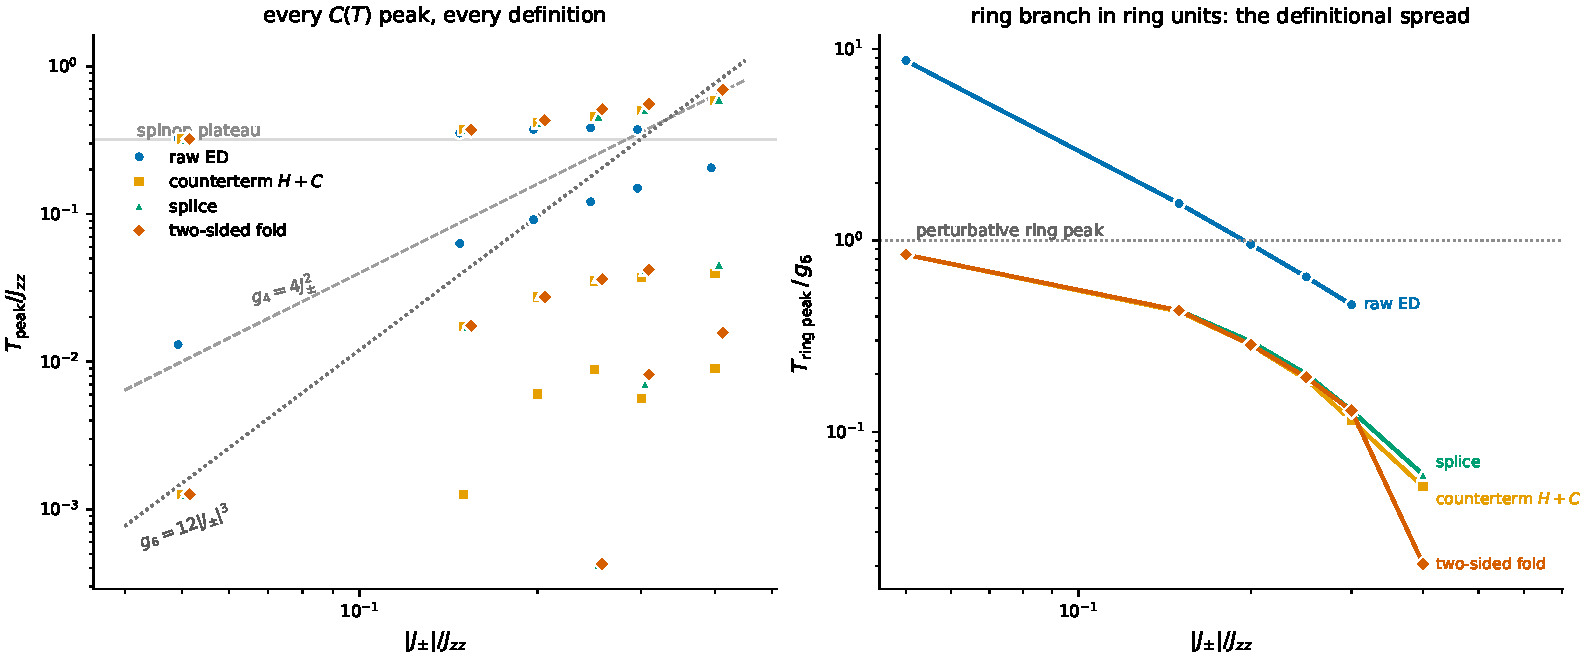
\includegraphics[width=\textwidth]{figs/fig_fold_peaks.pdf}
\caption{Every specific-heat maximum of every definition across the
coupling scan (left) and the ring branch in units of $\gsix$ (right).
Three branches organize the left panel: the spinon anomaly on top, the
ring branch below it, and a low-temperature third-peak branch that only
the winding-free definitions possess (Sec.~\ref{sec:thirdpeak}).  On the
ring branch, raw ED runs along the artifact scale $\gfour$ and crosses
$1\,\gsix$ near $-0.22$ purely by coincidence of scales; the three
winding-free definitions collapse onto a single curve through $-0.30$
($\sim$12\% spread in position) and fan out by a factor of three at
$-0.40$ (fold $0.020\,\gsix$, counterterm $0.052$, splice $0.060$) ---
the definitional ambiguity made visible.  At $-0.40$ raw ED has no
low-temperature peak at all: the artifact scale has grown into the
spinon scale and swallowed every gauge-sector feature, while the
winding-free definitions still resolve structure there.}
\label{fig:foldpeaks}
\end{figure}

Figure~\ref{fig:foldpeaks} condenses the whole scan into the peak
positions.  One reading caution that cost an afternoon: the campaign's
two-window peak extractor silently clips whichever maximum crosses its
$T=0.05$ split (strong-coupling raw ``peaks'' all read exactly $0.0497$
in the archived records); peak positions must be re-extracted as true
local maxima of the curves.  The ruler, audited again.

One thing this scheme does \emph{not} do is beat the obstruction theorem
--- nothing can.  The theorem's thermodynamic meaning is that
``winding-free'' is only exactly defined \emph{on the band}; any extension
to the full spectrum must decide which ninety full-space levels the band
replaces, and that decision is a convention of order $1-Z$.  The
counterterm, the splice, and the fold are therefore three
\emph{definitions} of the same non-unique reference.  They provably agree
at weak coupling (measured: exactly); their mutual spread at strong
coupling is not a defect of any one of them but the honest, irreducible
error bar on the concept of winding-free thermodynamics itself --- and
quoting that spread is the right practice.  The fold simply has the best
structural properties of the three: no anchor energy, no \emph{positional}
assignment (only a $Z$-ranking whose sharpness is itself measured), smooth
behavior through dissolution, and a path to larger clusters.

For completeness, the genuinely different roads, with their price tags:
\begin{center}
\small
\begin{tabular}{p{4.3cm}p{4.9cm}p{4.9cm}}
\toprule
\textbf{route} & \textbf{what it buys} & \textbf{what it costs}\\
\midrule
counterterm $H+C$ & complete spectrum from one solve & anchored at $z_0$;
residue grows as $1-Z$\\
splice & exact band $+$ full continuum & needs the band below the
continuum ($|\Jpm|\lesssim0.22$)\\
two-sided fold ($Z$-ranked) & no anchor, no positional assignment,
BICs slot in, survives dissolution, scalable & $O(1-Z)$ definitional
ambiguity (irreducible for anyone); the naive \emph{weighted} version
fails outright (hijacked ensemble)\\
NLCE on open clusters & winding loops \emph{never exist} --- no torus, no
artifact, by construction & converges only down to intermediate $T$; the
photon regime needs embedding orders far out of reach\\
girth-engineered cells & demotes the artifact itself to higher order in
$\Jpm$ & combinatorial search; the remedy shrinks the disease rather than
curing it\\
\bottomrule
\end{tabular}
\end{center}

The NLCE row deserves one sentence of emphasis: linked-cluster expansions
sum \emph{open} clusters, which have no glued edges and therefore no
winding loops at all --- the artifact this entire document fights simply
never appears.  That makes NLCE (a QED-backed tier of which already exists
in the parent codebase) the one fully independent cross-check of
winding-free thermodynamics in the temperature window where it converges;
it cannot reach the photon scale, but agreement in the overlap window is
evidence money cannot buy.  Perturbative subtraction of the artifact from
$\ln\mathcal{Z}$ order by order is also possible but adds nothing: it
works exactly where the counterterm already works, and fails where it
fails.

\subsection{The third peak: three bumps, one name}
\label{sec:thirdpeak}

Below the ring anomaly, $C(T)$ at strong coupling grows extra
low-temperature structure --- the ``third peak'' of
Sec.~\ref{sec:strong}'s lesson box and the lowest branch of
Fig.~\ref{fig:foldpeaks}.  Asking \emph{is it physical?} turned out to
have three different answers, because ``the third peak'' named three
different objects.  Untangling them is a case study in the campaign's
central habit: the exact masked spectrum is the referee.  A degeneracy it
declares exact must not radiate a heat-capacity bump; a gap it certifies
must.  Figure~\ref{fig:thirdpeak} demonstrates all three verdicts directly
from the computed spectra.

\begin{figure}[t]
\centering
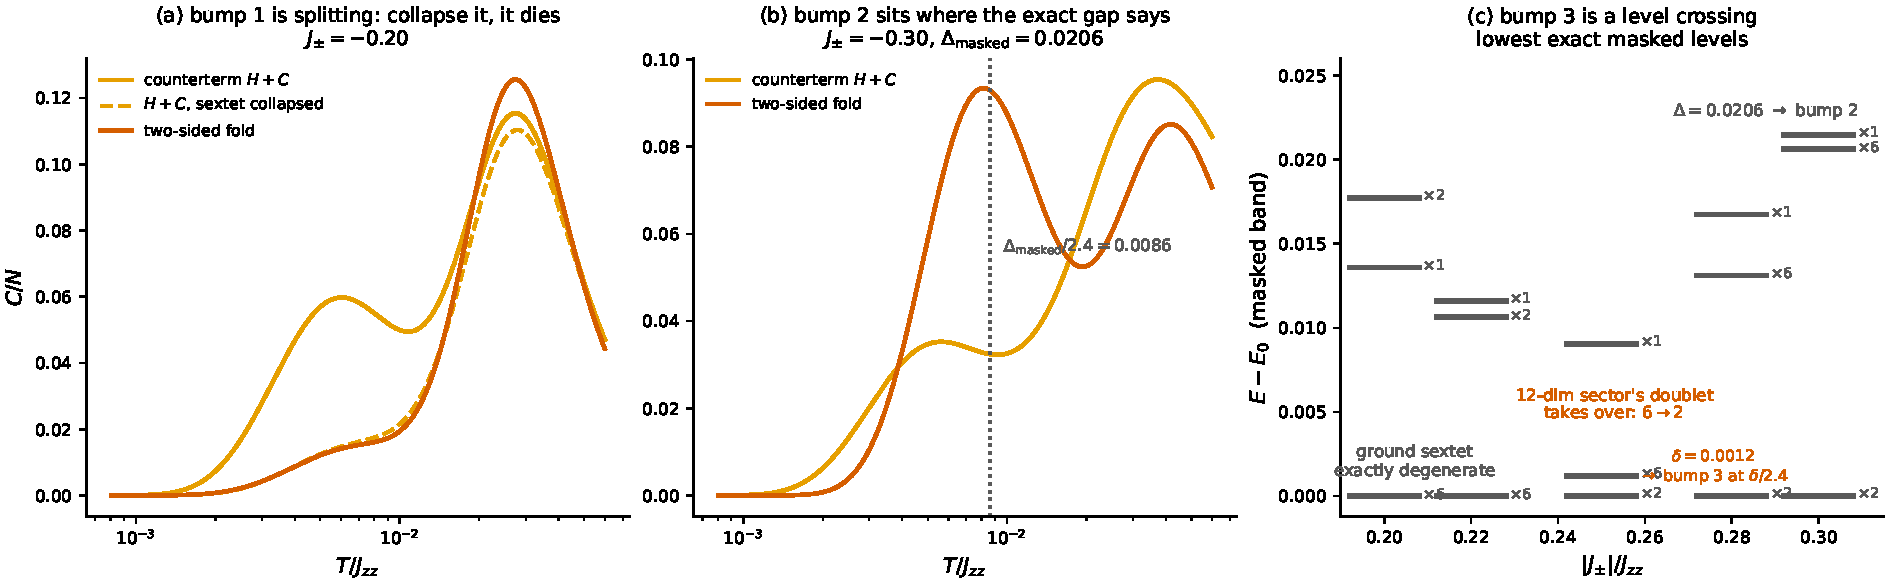
\includegraphics[width=\textwidth]{figs/fig_third_peak.pdf}
\caption{The third-peak taxonomy, demonstrated.  (a)~At $\Jpm=-0.20$ the
counterterm curve has a low-temperature bump the fold lacks; collapsing
the six lowest $H+C$ levels --- the image of the exactly-degenerate
masked ground sextet --- to their mean (dashed) kills the bump and lands
on the fold curve: bump~1 is pure multiplet splitting, the counterterm's
residue radiating.  (b)~At $\Jpm=-0.30$ the fold curve peaks at the
two-level Schottky position $\Delta_{\rm masked}/2.4=0.0086$ predicted
by the exact masked internal gap $\Delta=0.0206$: bump~2 is a certified
gap speaking.  (c)~The lowest exact masked levels versus coupling: the
ground sextet is degenerate to all digits through $-0.22$; at $-0.25$
the twelve-dimensional sector's doublet dives below it ($6\to2$),
leaving the splitting $\delta=0.0012$ whose Schottky at
$\delta/2.4\approx5\times10^{-4}$ is bump~3.}
\label{fig:thirdpeak}
\end{figure}

\begin{description}
\item[Bump 1: the counterterm's splitting bump --- artifact
(Fig.~\ref{fig:thirdpeak}a).]
In the exact masked map the sector ground states are \emph{exactly}
degenerate: six states, one per eight-dimensional transport sector, with
spread $0.00000$.  The counterterm splits them --- $C$ cancels transport
inside the ice block at one energy while $PHQ$ keeps transporting --- by
a fraction of the bandwidth growing from $0.011$ at $-0.10$ to $0.115$
at $-0.30$, and the split multiplet radiates a spurious Schottky bump.
These are the counterterm-\emph{only} peaks of
Fig.~\ref{fig:foldpeaks} (at $T=0.0013$ at $-0.15$, $0.006$ at $-0.20$),
absent from splice and fold, whose lowest levels are the exact masked
roots.  The surgical proof: keeping only the five lowest $H+C$ levels
reproduces the bump ($0.00548$ vs $0.00564$ at $-0.30$); collapsing
their splitting to zero removes it exactly.  Verdict: \textbf{not
physical} --- it is the $1-Z$ residue of Sec.~\ref{sec:hclimits} made
visible at low temperature.

\item[Bump 2: the internal-gap Schottky --- physical
(Fig.~\ref{fig:thirdpeak}b).]
The exact winding-free spectrum has a genuine gap between the
mask-protected ground multiplet and the seventh band level.  Two
independent constructions see the same number: at $-0.22$ the exact
masked gap is $0.010634$ and the counterterm's is $0.010730$.  At weak
coupling the resulting bump sits at $0.79\,\gsix$, indistinguishable
from the ring anomaly at $0.84\,\gsix$ --- it \emph{hides inside the
ring peak}; by $-0.22$ the two have separated by a factor of seven and
it becomes a visible third maximum.  At $-0.30$ the gap is $0.0206$ and
the fold and splice curves peak at $T\approx0.008\approx\Delta/2.4$, the
textbook two-level Schottky position --- and the fold's lowest levels
there \emph{are} the masked roots verbatim, so the feature is exact by
construction.  Verdict: \textbf{physical}.

\item[Bump 3: the multiplicity-change peak --- physical, and a free
diagnostic (Fig.~\ref{fig:thirdpeak}c).]  At $-0.25$ the ground multiplicity of the masked band
drops from six to two: the twelve-dimensional sector takes over the band
bottom, a level crossing \emph{within} the winding-free ground manifold.
The tiny exact splitting it leaves behind radiates the ultra-low maximum
at $T=4\times10^{-4}$ in the splice and fold curves at $-0.25$
(Fig.~\ref{fig:foldpeaks}, lowest points).  Verdict: \textbf{physical}
--- and useful: a heat-capacity fingerprint of ground-sector
reorganization, visible without ever inspecting an eigenvector.
\end{description}

Two honesty riders on the word ``physical''.  First, it means: a true
feature of the exact winding-free reference \emph{on this cluster}.
Whether the 16-site band's internal gap survives on FCC-32 --- sectors
forty times larger, flux unpinned --- is exactly the kind of question
the cluster, not the method, decides (Sec.~\ref{sec:cluster}).  This
rider has since been cashed for bump~3: the FCC-32 scan
(Sec.~\ref{sec:fcc32first}) finds \emph{no} multiplicity change at any
coupling, so the crossing --- and its little Schottky --- are real
physics of the 16-site torus and of nothing larger
(Sec.~\ref{sec:crossingmeaning} draws the moral).  Second,
at the couplings where the third peak stands separate, the definitional
spread of Fig.~\ref{fig:foldpeaks} is already growing; the peak's
\emph{existence} is definition-independent (its levels are sub-continuum
masked roots, exact and shared by every construction that inherits
them), but any statement about its precise \emph{lineshape} carries the
spread.

\begin{plainwords}
Same temperature window, three causes.  A counterterm error split an
exact degeneracy --- fake, and diagnosed because the exact masked
spectrum says those states are degenerate to all digits.  A real gap
inside the clean band --- real, certified by two independent
constructions agreeing on the gap to three digits.  And a change of
which sector owns the ground state --- real, and a bonus: the specific
heat announces the level crossing on its own.  The referee in every case
is the same: exact degeneracies must stay silent, certified gaps must
speak.
\end{plainwords}

\subsection{What the crossing means --- and what it does not}
\label{sec:crossingmeaning}

Bump 3 records a change in the ground-state multiplicity, and a level
crossing with a degeneracy change sounds like a phase transition.  It is
not one --- and what it actually is deserves care, because it is arguably
more interesting.

First, what it is not.  It is \emph{not} a ground-state level crossing of
the actual Hamiltonian: the raw ground state of this cluster evolves
smoothly and monotonically all the way to $\Jpm=-1$, with no crossing
anywhere.  The 6$\to$2 crossing lives in the winding-free band, and it is
a crossing between \emph{different transport sectors} --- the incoming
doublet belongs to the twelve-dimensional polarization sector, displacing
a sextet assembled from six eight-dimensional sectors.  Transport sectors
are not symmetry sectors of any local order parameter; they are the
\emph{topological} sectors of the emergent gauge field on the torus
(polarization is electric flux threading the handles,
Eq.~\ref{eq:rho}).  A change in which topological sector owns the ground
state is a reordering of flux-sector energetics: no local observable
jumps, nothing orders, no symmetry breaks.  On a single finite cluster,
that is spectroscopy, not a transition.

Here is why it is interesting anyway.  In a gauge theory, the energy
splittings between flux sectors are precisely the quantity whose
\emph{system-size scaling} diagnoses the phase (the 't~Hooft criterion
--- and the reason Sec.~\ref{sec:roadahead} insists the masked-out
sectors be recycled, not discarded): in the photon phase the splittings
must vanish as the torus grows; in a Higgs or confined regime they
saturate.  The crossing is a single data point of exactly the right
diagnostic, waiting for a size axis.

And it sits at a suspicious address.  The crossing lands at
$\Jpm=-0.25$ --- the coupling where one line of theory (the
self-consistent exclusion-boson treatment) predicts the $\pi$-flux
spin-ice phase terminates, $\Jpm/\Jzz=-1/4$; a competing estimate puts
the terminus near $-0.5$.  It is also where the masked band's
completeness begins to degrade.  So a tempting reading exists: \emph{the
6$\to$2 crossing is the finite-size shadow of the QSI terminus} --- the
gauge theory's sector energetics inverting as the Higgs frontier
approaches.  Three caveats before believing it: cubic-16's ground-state
flux is pinned by pure counting, so its sector energetics are partly
arithmetic; the splitting is tiny ($0.0012\,\Jzz$) and must sharpen, not
vanish, with system size to mean anything; and the definitional spread
is already growing there (though the crossing itself is between
sub-continuum masked roots --- exact and shared by every construction).

Is it still a spin liquid beyond?  What theory requires: the deconfined
phase is a genuine phase --- the photon either exists or it does not ---
so a true $T=0$ transition out of it must occur \emph{somewhere} in the
thermodynamic limit.  Beyond it, though, no further sharp structure is
required: the spinons carry fundamental gauge charge, so the Higgs and
confined regimes are smoothly connected to each other
(Fradkin--Shenker), consistent with the continuous dissolution we
measure.  What this cluster sees: every gauge signature fades smoothly
--- the flux expectation from $-0.25$ at weak coupling to $-0.067$ at
$-0.30$ and $-0.009$ at $-0.35$, the ring scale renormalized to
$\sim0.1\,\gsix$, the purity to $Z\approx0.25$ --- with no condensation,
no symmetry breaking, no raw-level crossing.  That is exactly what a
true transition \emph{rounded by a tiny torus} looks like, and also
exactly what a crossover looks like; sixteen sites cannot tell them
apart.  Best current statement: the terminus lies somewhere in
$[-0.25,-0.5]$, and this cluster cannot adjudicate.

Two measurements would decide it.  (i)~Does the crossing reproduce on
FCC-32 --- flux unpinned, sectors up to dimension 396 --- and does its
coupling converge with cluster size and truncation depth?  A physical
terminus shadow drifts systematically; an artifact wanders or vanishes.
(ii)~The flux-sector splitting scaling itself, across sizes and girths.

\textbf{Measurement (i) has now been made
(Sec.~\ref{sec:fcc32first}), and the answer is: it vanishes.}  On
FCC-32 the band bottom belongs to the unique largest
(zero-polarization) sector at \emph{every} coupling from $-0.05$ to
$-0.32$, with a twelve-fold degenerate multiplet of 140-dimensional
sectors above it and a gap that only grows --- and deepening the
truncation from $L=1$ to $L=2$ \emph{entrenches} that ordering (the
gap at $-0.22$ triples), the opposite of what a hidden crossing would
do.  This is exactly the ordering the photon phase predicts: flux
costs energy, so the zero-flux sector sits lowest.  The correct
reading of cubic-16's crossing is therefore deflationary: its
pathological sector structure (flux pinned by counting, sectors of
dimension at most twelve) put the \emph{wrong} sectors on the bottom
at weak coupling, and the celebrated 6$\to$2 crossing at $-0.25$ was
the small cluster relaxing into the correct ordering --- a cluster
artifact, not a terminus shadow.  The coincidence with the
$-1/4$ prediction was a coincidence.  Bump~3 of the taxonomy is
correspondingly a cubic-16-only feature, exactly the outcome its
cluster rider anticipated.

What survives, sharpened: the terminus question itself now rests
entirely on measurement (ii) --- the sector splittings, measured on
both clusters and growing smoothly with coupling, are the raw material
of the 't~Hooft scaling analysis, and the recycled-sector program of
Sec.~\ref{sec:roadahead} remains the road to it.  And there is a
methodological moral worth stating plainly: the machinery in this
document not only found a sharp feature, it then \emph{killed its own
most exciting interpretation} with a controlled measurement on a
better cluster.  That is what the validation-first culture of this
campaign is for.

\begin{lesson}
\textbf{Repairs that are not repairs.}  Two tempting improvements were
tested and made things \emph{worse}.  (i) Forcing the upper $H+C$ band to
inherit the exact degeneracy pattern of the masked map (``sector
symmetrisation'') increased the error everywhere --- the pattern is exact
but the eigenvectors are not, so the symmetrisation imposes structure the
true operator does not have.  (ii) Hand-built counterterms from a catalogue
of loop shapes missed whole classes of winding processes and shifted the
\emph{physical} part of the map by up to $42\%$.  Moral: a correction must
be derived from the exact object ($F$ itself), not from a plausible model of
it.
\end{lesson}

\begin{lesson}
\textbf{Estimator traps.}  Three measurement bugs each briefly masqueraded
as physics.  (i) A comparison routine silently \emph{shifted} one spectrum
to match the mean of another --- invisible in level differences, corrupting
every absolute-energy comparison.  (ii) Classifying $C(T)$ peaks by
Boltzmann weights mislabels them; the correct weight is each level's share
of the heat-capacity \emph{variance}.  (iii) The entropy sum rule
$\int C/T\,dT=\ln 2$ converges like $1/T_{\max}^2$: truncating at
$T_{\max}=60$ leaves a deficit that looks exactly like a lost energy level
and does not improve with grid refinement.  ($T_{\max}=600$ resolves it.)
Moral: before blaming the physics or the method, audit the ruler.
\end{lesson}

%=====================================================================
\section{Turning the second dial: what $\Jpmpm$ actually does}
\label{sec:jpmpm}

Everything so far lived on the XXZ line, where the only transverse coupling
is $\Jpm$.  There the two anomalies of $C(T)$ sit absurdly far apart: at
$\Jpm=-0.125$ the winding-free gauge peak is at $0.0121\,\Jzz$ and the
spinon peak at $0.274\,\Jzz$, a ratio of $0.044$ --- a factor of
twenty-three.  The real materials refuse to behave: Ce$_2$Hf$_2$O$_7$ shows
two heat-capacity anomalies at $65$ and $24$~mK, a ratio near $0.37$.  A
factor of twenty-three against a factor of under three is not a discrepancy
to be split; it is a different picture of the world.

The obvious suspect is the coupling we had switched off.  Real cerium
pyrochlores are XYZ, and in the $\Jpm$ language that means a second
transverse term, the \emph{pair flip} $\Jpmpm$, which flips two spins the
\emph{same} way instead of exchanging them.  It is not small in the fits:
for the published Ce$_2$Hf$_2$O$_7$ parameters $\Jpmpm$ is comparable to
$\Jpm$ itself.  So we turned the dial --- an $8\times7$ grid, $56$ cells,
each one a complete exact band --- and asked whether it closes the gap.

\subsection{What a pair flip costs}

Start with what the move does to the ice rules, because that sets
everything else.

\begin{worked}
Take a tetrahedron obeying two-in--two-out, so its charge is $Q_t=0$, and
recall the energy is $\tfrac12\sum_t Q_t^2$ in units of $\Jzz$.

\emph{An exchange move} ($\Jpm$) flips one up and one down spin on a bond.
The tetrahedron containing both keeps two ups: $Q_t=0$, no cost.  The two
outer tetrahedra --- one for each flipped site --- gain and lose one
respectively: $Q=\pm1$, costing $\tfrac12$ each.  \textbf{Total: one unit.}
That is a spinon--antispinon pair, the familiar excursion.

\emph{A pair flip} ($\Jpmpm$) flips two spins that were both pointing the
same way.  Now the shared tetrahedron goes from two ups to four:
$Q_t=+2$, costing $\tfrac12(2)^2=2$.  The two outer tetrahedra each gain
one: $\tfrac12$ each.  \textbf{Total: three units.}
\end{worked}

So a pair flip is three times as expensive as an exchange, and it is
\emph{qualitatively} different: it manufactures a \textbf{double monopole},
a tetrahedron carrying twice the elementary gauge charge, flanked by two
ordinary spinons.  It also fails to conserve the total $S^z$, which is why
the calculations in this section need the full $65\,536$-state space rather
than the $12\,870$-state sector the XXZ line lives in.

One thing does \emph{not} change.  The emptiness theorem of
Sec.~\ref{sec:emptyblock} survives verbatim: a pair flip acting on an ice
state always breaks the ice rule, so $PHP$ is still exactly diagonal ---
we checked it numerically, and it is zero to the last bit.  $\Jpmpm$ buys
no new direct ice-to-ice matrix element.  Whatever it does to the gauge
physics, it does through the resolvent, like everything else.

\subsection{Three measured effects, and a squeeze}

With the complete band in hand at every cell, three things happen as
$\Jpmpm$ is turned up at fixed $\Jpm$.  The numbers below are at
$\Jpm=-0.125$, the coupling closest to the Ce$_2$Hf$_2$O$_7$ fits, as
$\Jpmpm$ runs from $0$ to $0.30$.

\begin{enumerate}
\item \textbf{The band sinks.}  Its bottom drops from $-0.437\,\Jzz$ to
$-0.822\,\Jzz$.  This is ordinary variational bookkeeping: expensive as
they are, virtual pair excursions are extra ways for the ice states to
lower their energy, and more channels always means a deeper ground state.
\item \textbf{The band widens} --- from $0.075\,\Jzz$ to $0.184\,\Jzz$,
a factor of $2.5$.  The gauge peak tracks the bandwidth, so it rises:
$0.0121 \to 0.0185\,\Jzz$, up $53\%$.  The photon gets \emph{faster}.
\item \textbf{The spinon scale softens} --- the upper peak falls
$0.274 \to 0.168\,\Jzz$, down $39\%$.  Pair flips help the spinon
continuum more than they help the band, because a region already full of
monopoles has far more ways to use them, so the continuum descends faster
than the band does and the gap between them closes from above.
\end{enumerate}

The two peaks therefore approach each other \emph{from both sides at once}:
the gauge anomaly climbing, the spinon anomaly sinking.  The ratio duly
improves, $0.044 \to 0.110$.

\begin{plainwords}
Think of the two peaks as two shelves, one very low and one high, and you
are trying to bring them together.  Turning up $\Jpmpm$ raises the low
shelf and lowers the high one simultaneously --- exactly the move you
wanted.  It works.  It just does not work anywhere near hard enough: the
shelves close from a factor of twenty-three to a factor of nine, and the
experiment wants a factor of three.
\end{plainwords}

\subsection{Why it stops: the dial destroys what it moves}

The squeeze does not gently saturate --- it terminates, and for a reason
that is inevitable in hindsight.

The mechanism by which $\Jpmpm$ closes the gap \emph{is} the admixture of
non-ice configurations into the band.  The ice weight $Z$
(Sec.~\ref{sec:feshbach}: the fraction of a level living inside the ice
manifold) measures exactly
that admixture, and it decays as the dial turns: at $\Jpm=-0.125$ the
median $Z$ slips from $0.723$ to $0.640$; at $\Jpm=-0.20$, from $0.497$ to
$0.257$.  Push further and there is nothing left to speak of.  At
$(\Jpm,\Jpmpm)=(-0.05,0.30)$ only $25$ of the $90$ levels survive as band
states at all and the largest ice weight anywhere is $0.001$ --- the band
has dissolved completely.

That corner is worth naming precisely, because it is the one place in the
plane where dissolution is real rather than instrumental.  It is not set by
$|\Jpm|$, the dial that governs dissolution on the XXZ line.  It is set by
the \emph{ratio}: the band dies when $\Jpmpm/|\Jpm| \gtrsim 5$.  At
$\Jpm=-0.05$ that threshold is crossed by $\Jpmpm=0.25$ (marginal, $86/90$)
and comprehensively by $0.30$; at $\Jpm=-0.20$, where the same $\Jpmpm=0.30$
is only $1.5$ times the exchange, the band is intact at $90/90$.  When the
pair term dominates the exchange term outright, the ice manifold stops being
the right low-energy description --- and no amount of careful bookkeeping
about winding loops can rescue a band that is no longer there.

So the two effects are the same effect wearing different hats.  You close
the gap by dressing the band with monopoles; dress it enough and you have
destroyed the band.  The best ratio in the whole plane, $0.1216$ at
$(-0.16,0.30)$, sits exactly where you would expect from that
trade-off: at intermediate exchange, with the pair term pushed as far as
the band will tolerate and not one step further.

\subsection{The verdict, and one honest complication}

The ceiling over all $56$ cells is $\mathbf{0.1216}$, against a measured
$0.37$.  $\Jpmpm$ moves the ratio by a factor of about $2.5$ and needs a
factor of eight.  \textbf{On the 16-site cell, the second dial does not
rescue the peak separation.}  Combined with the cluster comparison of
Sec.~\ref{sec:cluster} --- where FCC-32 pushes the ring peak
\emph{further} down, to $0.29\,\gsix$ against cubic-16's $0.84$ --- the
honest reading is that the $24$~mK anomaly in Ce$_2$Hf$_2$O$_7$ is probably
not the photon peak at all.

The complication is a second kind of merging, and it is real.  At strong
exchange and large pair coupling --- nine cells with $|\Jpm|\ge0.20$ ---
the gauge peak and the sub-gauge peak of Sec.~\ref{sec:thirdpeak} run
together into a single maximum.  At $(-0.27,0.20)$ there is one sub-spinon
maximum at $0.0121\,\Jzz$ where both neighbours in $\Jpmpm$ carry two, near
$0.005$ and $0.039$.  This is a genuine merge of two low-temperature
features; it is \emph{not} the gauge peak meeting the spinon peak, and it
moves the ratio the wrong way, down to $0.028$--$0.045$.  Any convention
that reports ``the highest maximum below the spinon split'' will report the
merged position and produce a branch that appears to jump.  It jumps
because the peaks merged, not because the tracking failed.

\begin{lesson}
An earlier pass over this plane reported a ratio of $0.332$ at
$(-0.125,0.30)$ --- tantalisingly close to experiment, and wrong.  The
anchor solve had found only $27$ of the $90$ band levels there, and the
two-sided fold removes exactly as many raw levels as it has replacements
for.  So $63$ ice-descended raw levels stayed in the ensemble \emph{beside}
their own replacements, and the low-temperature peak was radiating from the
double-counted remainder.  With the complete band the same cell reads
$0.110$.

The diagnosis is worth keeping, because the failure was silent: every
individual number was computed correctly.  Two habits catch it.  First,
a fold that replaces a band must replace \emph{all} of it or refuse to run
--- a partial replacement is not a weaker result, it is a different and
meaningless one.  Second, when an instrument is upgraded, re-run the cells
where the old one \emph{succeeded}: the bordered solver reproduces the
old ratios to the digit wherever the old band was complete
($(-0.20,0.15)$: $0.0893 \to 0.0893$), which is what makes the changes
elsewhere trustworthy rather than merely different.
\end{lesson}

%=====================================================================
\section{What the campaign established}
\label{sec:results}

A compact scoreboard of the physics results, all on the 16-site cell unless
stated:

\begin{itemize}
\item \textbf{Naive ED never measures the photon.}  Its low-$T$ peak tracks
the artifact scale $\gfour$ (exponent $1.99\approx2$); against the photon
scale it drifts by a factor 40.  The winding-free peak tracks $\gsix$
(exponent $3.10\approx3$) and approaches $1.02\,\gsix$ as $\Jpm\to0$ --- the
perturbative prediction, recovered exactly where it must hold.
\item \textbf{Flux-sign physics is real and restored:} $\pi$-flux
suppression versus zero-flux enhancement of the ring scale
(e.g.\ $0.73\,\gsix$ vs $1.13\,\gsix$ at $|\Jpm|=0.046$), with the correct
sign of the hexagon expectation at every coupling --- naive ED gets the sign
wrong everywhere.
\item \textbf{The spinon peak is robust:} identical (4 digits) between naive
and winding-free treatments up to $|\Jpm|\approx0.07$ --- as it must be,
since spinons live outside the ice manifold.  A method that ``cleans'' the
spinon peak would be destroying physics; this one provably does not touch it.
\item \textbf{The photon does not decay} in the winding-free world:
all masked levels have zero width at every coupling tested; apparent
band merging in naive ED is frame artifact.  Escaped levels at
$|\Jpm|\ge0.24$ are bound states in the continuum, protected by transport
symmetry.
\item \textbf{A third, physical Schottky peak} exists at $|\Jpm|\ge 0.22$
from a genuine internal gap of the winding-free spectrum.
\item \textbf{Application to Ce$_2$Hf$_2$O$_7$:} at literature couplings the
naive ED peak lands deceptively close to the measured 24\,mK anomaly ---
but the winding-free calculation shows that agreement is a coincidence
between the \emph{artifact} scale and the data; the true ring peak on this
cell is at 6\,mK.  A cautionary tale for fitting experiments with naive
small-cluster ED.
\item \textbf{Dissolution is continuous:} band isolation is lost at
$\Jpm\approx-0.185$, completeness degrades from $-0.24$, and by $-0.30$ the
band is as wide as the spinon scale.  No sharp wall, no phase transition of
the ground state --- and the strong-coupling interpretation (Higgs frontier
of the emergent gauge theory) is the subject of the follow-up project.
\end{itemize}

%=====================================================================
\section{The cluster is the error bar}
\label{sec:cluster}

With the artifact provably removed, what limits accuracy?  The box itself
--- but now in the ordinary, honest way: through what it can and cannot
represent.  The comparison between the two available cells is stark:

\begin{center}
\begin{tabular}{lcc}
\toprule
 & cubic 16-site & FCC 32-site\\
\midrule
ice states & 90 & 2970\\
transport sectors & 25 & 85\\
largest sector & 12 & 396\\
flippable hexagons per state & 0 or 4 only & 0, 4, 6, 7, 8\\
ground-state flux & \emph{pinned by counting} & free\\
winding-free ring peak at $\Jpm=-0.05$ & $0.84\,\gsix$ & $0.29\,\gsix$\\
\bottomrule
\end{tabular}
\end{center}

A factor of \emph{three} in the headline number, between two clusters with
the identical, exact protocol.  The 16-site cell is simply a poor host: its
ice manifold is so small that the flux is fixed by arithmetic before any
dynamics happens.  This is the single most important systematic in the whole
program, and it motivates everything in the final section.

\subsection{First steps onto FCC-32: calibrate, then scale}
\label{sec:fcc32first}

The crossing question of Sec.~\ref{sec:crossingmeaning} forces the move
to FCC-32, and the move immediately raises a practical wall: the
$S^z=0$ block there has 601 million states.  The Feshbach fold's escape
hatch is \textbf{graded truncation}: keep only the spinon states
reachable from the ice manifold in at most $L$ pair-flip moves.
Physically, $L$ is \emph{how deep a virtual spinon excursion the
calculation can follow before being forced home} --- one freshly created
adjacent pair at $L=1$; the pair separated, or a second pair, at $L=2$;
and so on.  Since strong-coupling dressing \emph{is} spinons wandering
far and often, $L$ is the convergence dial of everything on the large
cluster, and its ladder is the error bar.

\begin{lesson}
\textbf{The instrument that failed its physical.}  A truncated FCC-32
band pipeline already existed (one-pair truncation, map evaluated at a
single anchor energy), and the obvious plan was to simply run it near
the crossing.  Calibrating it first on cubic-16 --- where the exact
answer is known --- stopped that: it shows \emph{no crossing at all},
even at $-0.30$, with multiplet gaps wrong by a factor of four.  The
fixed anchor misses the self-consistent $\sim\!Z$ renormalization of
level spacings.  Run uncalibrated, it would have returned a confident,
wrong verdict on precisely the question at stake.  Rule: an instrument
earns the big cluster only by first reproducing known truth on the
small one.
\end{lesson}

The instrument that passes: each sector's masked spectrum is exactly the
spectrum of the Hermitian \emph{bordered matrix}
$M_s = \begin{pmatrix}(PHP)_{ss} & (PHQ)_s\\ (QHP)_s & QHQ\end{pmatrix}$
(the same object that explained the BICs in
Sec.~\ref{sec:bic}), so sparse Lanczos on $M_s$ delivers each sector's
ground energy with \emph{no anchor and no self-consistency loop} ---
exact within the truncation.  Its cubic-16 ladder, against the known
crossing:

\begin{center}
\small
\begin{tabular}{cccl}
\toprule
$L$ & truncated space & cost & crossing verdict\\
\midrule
1 & 1\,242 & instant & absent, even at $-0.30$ --- fails\\
2 & 5\,754 & instant & present, displaced into $(-0.25,-0.30)$\\
3 & 11\,130 & seconds & present, within $\sim0.02$ of the true coupling\\
4 & 12\,870 ($=$ full) & seconds & \textbf{exact to all digits}\\
\bottomrule
\end{tabular}
\end{center}

Monotone convergence from below, with the crossing coupling drifting
systematically toward truth --- so on FCC-32 the drift between $L$
levels is a measured error bar, not a hope.  The FCC-32 costs, measured
on the campaign machine: $L=1$ has 140\,442 states (seconds per
sector); $L=2$ has 2\,511\,450 states, a 50-million-element sparse
Hamiltonian built in 12 seconds, and one sector ground in 154 seconds
--- about 3.6 hours per coupling for all 85 sectors; $L=3$ fits in
memory but costs roughly a day per coupling, reserved for single-point
convergence checks.

The scans are done, and the result is unambiguous.  FCC-32's 2\,970 ice
states split into 85 sectors with dimensions
$1{\times}396$, $12{\times}140$, $6{\times}72$, $24{\times}12$,
$12{\times}6$, $24{\times}4$, $6{\times}1$.  At \emph{every} coupling
scanned ($L=1$: thirteen points, $-0.05$ to $-0.32$; $L=2$: four
points), the band bottom belongs to the unique 396-dimensional
zero-polarization sector, with the twelve 140-dimensional sectors
forming an exactly degenerate runner-up multiplet:

\begin{center}
\small
\begin{tabular}{lcccc}
\toprule
gap to runner-up multiplet & $-0.05$ & $-0.22$ & $-0.26$ & $-0.30$\\
\midrule
$L=1$ & $0.0014$ & $0.0137$ & $0.0164$ & $0.0191$\\
$L=2$ & $0.0018$ & $0.0374$ & $0.0473$ & $0.0573$\\
\bottomrule
\end{tabular}
\end{center}

No crossing, anywhere --- and the truncation trend runs \emph{opposite}
to a hidden one: going deeper ($L=1\to2$) makes the zero-polarization
sector's dominance stronger, where on cubic-16 going deeper is what
\emph{revealed} the crossing.  The verdict this feeds is drawn in
Sec.~\ref{sec:crossingmeaning}.  (Measured runtimes for the record:
$1.6$--$2.9$ hours per $L=2$ coupling --- the weak-coupling points
converge fastest.)

Honesty about what FCC-32 will and will not deliver.  The sector-ground
scan answers the crossing question.  The full \emph{peak} program needs
the entire 2\,970-level winding-free band, and there the estimator
ladder currently reads: full self-consistency --- validated excellent
on cubic-16 (ring peak to $0.3\%$ at $L=3$) --- is unaffordable on
FCC-32; the cheap single-anchor slope correction lands $7$--$14\%$ high
on the ring peak; and a naive multi-anchor version is \emph{unstable} at
strong coupling (anchors placed near the descended continuum corrupt
the branch assignment --- measured, not conjectured).  A branch-tracked
multi-anchor root finder is the one named engineering gap between here
and the full peak scan on FCC-32.  And two things never come from
FCC-32 at all: the raw-ED comparison curve and the spinon anomaly, both
of which need the 601-million-level spectrum --- those remain cubic-16
deliverables, which is an acceptable division of labor since every peak
that matters at strong coupling (ring, third, crossing) is
band-derived.

%=====================================================================
\section{The road ahead: beating finite size at strong coupling}
\label{sec:roadahead}

The next campaign asks: \emph{how do we maximally negate the remaining
finite-size effects, in the strong-coupling regime, without introducing new
physics or killing real physics?}  The answer designed above rests on a
diagnosis: at strong coupling the dominant box effect is no longer one thing
but three, and each has exactly one clean remedy.

\subsection{Residual 1: topology --- already solved}

The winding artifact itself is handled by the mask, which is combinatorial
and coupling-independent: it works identically at $\Jpm=-0.30$ and $-0.03$.
Nothing new needed --- but everything below must be built \emph{on top of}
the masked map, never instead of it.

\subsection{Residual 2: matched winding pairs --- solved by geometry}

Processes that wind $+1$ then $-1$ (net zero) are topologically trivial: no
label can see them, and the mask correctly keeps them.  At weak coupling
they are negligible (they cost two powers of the already-small winding
amplitude); at strong coupling they are not.  The \emph{only} knob is
geometry: their size is set by the length of the shortest winding loop the
cell permits.  Hence \textbf{girth engineering}: among all simulation cells
of a given size (including skewed, non-rectangular ones), choose the cell
that maximizes the shortest wrap-around ice loop.

\begin{figure}[h]
\centering
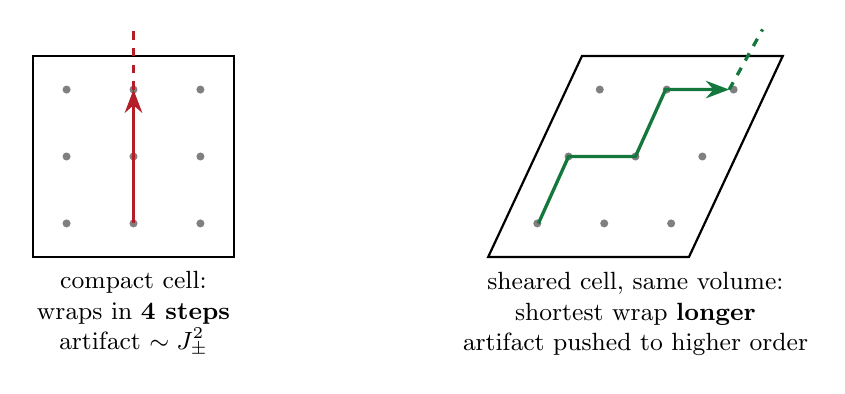
\begin{tikzpicture}[scale=0.85,>=Stealth]
% left: square cell, short wrap
\begin{scope}
\draw[thick] (0,0) rectangle (3,3);
\foreach \x in {0.5,1.5,2.5} \foreach \y in {0.5,1.5,2.5} \fill[black!50] (\x,\y) circle (0.06);
\draw[badcol,very thick,->] (1.5,0.5) -- (1.5,2.5);
\draw[badcol,very thick,dashed] (1.5,2.5) -- (1.5,3.4);
\node[font=\small,align=center] at (1.5,-0.85) {compact cell:\\ wraps in \textbf{4 steps}\\ artifact $\sim\Jpm^{2}$};
\end{scope}
% right: sheared cell, long wrap
\begin{scope}[xshift=6.8cm]
\draw[thick] (0,0) -- (3,0) -- (4.4,3) -- (1.4,3) -- cycle;
\foreach \x in {0.5,1.5,2.5} \foreach \y in {0.5,1.5,2.5}
  \fill[black!50] ({\x+0.4667*\y},\y) circle (0.06);
\draw[goodcol,very thick,->] (0.75,0.5) -- (1.2,1.5) -- (2.2,1.5) -- (2.65,2.5) -- (3.6,2.5);
\draw[goodcol,very thick,dashed] (3.6,2.5) -- (4.1,3.4);
\node[font=\small,align=center] at (2.2,-0.85) {sheared cell, same volume:\\ shortest wrap \textbf{longer}\\ artifact pushed to higher order};
\end{scope}
\end{tikzpicture}
\caption{Girth engineering.  The irreducible (net-zero-winding) artifact is
controlled by the length of the shortest wrap-around loop.  Skewing the
simulation cell at fixed size can lengthen that loop, demoting the residual
artifact by powers of $\Jpm$ --- at zero cost in Hilbert-space size.  The
search over cell shapes is purely combinatorial (no diagonalization needed).}
\label{fig:girth}
\end{figure}

Because the loop census is a counting exercise, thousands of candidate cell
shapes can be screened without a single diagonalization, scoring each by:
shortest winding loop (maximize), number of contractible hexagons (keep),
flippability variety (keep), flux unpinned (require), largest transport
sector (keep tractable).

\subsection{Residual 3: the coarse spinon continuum --- solved by twists,
reborn}

At strong coupling every low-energy state is heavily dressed by spinon
excursions ($1-Z$ up to $0.75$), but the small box offers only a handful of
discrete spinon levels where the infinite crystal has a dense continuum.
This misplaces the continuum edge, exaggerates the sharpness of the
dissolution, and expels the bound-in-continuum levels.

Here twist averaging returns --- in the \emph{opposite} role from
Section~\ref{sec:twist}.  Threading a flux shifts the spinon levels;
averaging over many twist values sweeps them across the true continuum,
exactly the classic ``boundary-condition integration'' of electronic
structure theory.  Crucially, the mask is applied \emph{at each twist}
(the transport label does not depend on the twist), so topology removal and
continuum densification never compete:

\begin{center}
\emph{mask handles the loops; twists handle the levels.}
\end{center}

\begin{figure}[h]
\centering
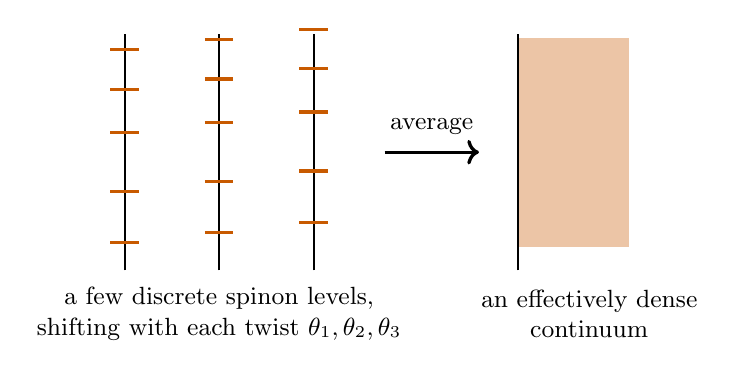
\begin{tikzpicture}[scale=1.0]
\foreach \i/\xs in {0/0.0,1/1.2,2/2.4}{
  \draw[thick] (\xs,0) -- (\xs,3);
  \foreach \y in {0.35,1.0,1.75,2.3,2.8}{
    \draw[spincol,very thick] ({\xs-0.18},{\y+0.13*\i}) -- ({\xs+0.18},{\y+0.13*\i});
  }
}
\node[font=\small,align=center] at (1.2,-0.55) {a few discrete spinon levels,\\ shifting with each twist $\theta_1,\theta_2,\theta_3$};
\draw[->,very thick] (3.3,1.5) -- (4.5,1.5);
\node[font=\small,above] at (3.9,1.6) {average};
\fill[spincol!35] (5.0,0.3) rectangle (6.4,2.95);
\draw[thick] (5.0,0) -- (5.0,3);
\node[font=\small,align=center] at (5.9,-0.55) {an effectively dense\\ continuum};
\end{tikzpicture}
\caption{The twist reborn.  Each twist value slides the discrete spinon
levels; averaging the \emph{masked} results over twists reconstructs a dense
continuum for the virtual excursions --- correct dressing, smooth continuum
edge --- without adding any new operator to the Hamiltonian.  Each twisted
problem is an exact microscopic Hamiltonian, so no physics is invented.}
\label{fig:densify}
\end{figure}

A free diagnostic comes along: genuine contractible physics is provably
twist-independent, so the \emph{spread} of the masked results across twists
is a direct, honest error bar on whatever finite-size effect remains.  And a
second dividend: a trustworthy continuum edge is exactly what the
bound-state-versus-resonance verdicts of Sec.~\ref{sec:bic} hinge on --- on
a coarse, undensified continuum, the question ``did this level really
escape?'' is not even well-posed.

\subsection{Honesty items}

Three more commitments, so the method neither invents nor kills physics at
strong coupling:
\begin{itemize}
\item \textbf{Graded truncation.}  On the 32-site cell the spinon space must
be truncated (one pair, two pairs of spinons).  At strong coupling the
one-pair truncation is not obviously sufficient; the protocol requires the
one-pair/two-pair difference to be measured and quoted at every coupling.
\item \textbf{Recover, don't repair.}  Where winding-free levels escape into
the continuum, they are recovered as symmetry-protected bound states (per
transport sector), not patched with counterterms.  Where the continuum in
the \emph{same} sector genuinely touches a level, its decay width is
computed and reported as physics --- at strong coupling a finite photon
lifetime, if real, must be allowed to appear.
\item \textbf{Recycle the removed sectors.}  The masked-out winding sectors
are not garbage: their energy splittings versus twist and cell size are
precisely the flux-sector free energies whose scaling distinguishes the
photon phase from a Higgs phase.  The artifact we negate in the physical
sector becomes the measurement in the diagnostic sector --- one production
run serves both this program and the strong-coupling phase-diagram project.
\end{itemize}

\subsection{The validation ladder}

Every stage of the new protocol must pass, in order:
\begin{enumerate}
\item \textbf{Weak-coupling anchor:} ring peak $\to\gsix$ with exponent 3 as
$\Jpm\to0$ on the new cell (the exact perturbative limit).
\item \textbf{Spinon neutrality:} the spinon peak agrees with naive ED at
weak coupling to 4 digits (the mask must not touch it).
\item \textbf{Flux law:} correct $\pi$-flux sign, and the known
flux-asymmetry between $\pm\Jpm$ at matched magnitude.
\item \textbf{Physical features survive:} the third Schottky peak present;
no feature removed that the exact masked reference possesses.
\item \textbf{Sum rule:} entropy integral returns $\ln 2$ (with the
$T_{\max}$ lesson applied).
\item \textbf{Cross-size consistency:} dimensionless ratios
(peak$/\gsix$, gaps$/\gsix$) drift monotonically and modestly from 16
$\to$ 32 $\to$ girth-optimized cells, with twist-spread error bars quoted.
\end{enumerate}

%=====================================================================
\section{Where the method ends: the Heisenberg point, and beyond}
\label{sec:heisenberg}

Every method should be able to say where its own writ runs out.  For the
mask the answer is unusually crisp --- and it is \emph{not} at the band
dissolution.  Dissolution only changes which instrument carries the load
(Secs.~\ref{sec:bic} and~\ref{sec:hclimits}).  The genuine boundary lies
deeper in coupling, at a point of enhanced symmetry.

\subsection{The Heisenberg point}

Our transverse term is $-\Jpm(S^+S^-+S^-S^+) = -2\Jpm(S^xS^x+S^yS^y)$, so
at
\[
\Jpm \;=\; -\tfrac12\,\Jzz
\]
the Hamiltonian becomes $\Jzz\,\mathbf{S}_i\cdot\mathbf{S}_j$: the
antiferromagnetic \textbf{Heisenberg} model, with full rotational (SU(2))
symmetry --- no direction in spin space is special anymore.  The campaign's
reconnaissance stopped at $\Jpm=-0.30$, well short of this point, and the
trend at the frontier was already steep: purity $Z\approx0.25$ and falling,
thirteen of ninety band levels escaped.

Two different things fail as this point is approached, and separating them
is the whole insight:

\begin{enumerate}
\item \textbf{Quantitatively, nothing crashes.}  $F(z)$ is linear algebra
on spin patterns; it exists at any coupling, and every self-consistent root
of the \emph{unmasked} map is an exact eigenvalue of $H$ no matter how
small $Z$ becomes.  The machinery runs at $-0.5$ as happily as at $-0.05$.
\item \textbf{Structurally, the mask breaks the symmetry.}  The transport
label is built on the ice manifold \emph{in the $S^z$ basis}.  At the
Heisenberg point the choice of $z$-axis is pure convention --- so ``the
winding-free model'' built on the $z$ basis and the one built on the $x$
basis are \emph{different operators with different spectra}, disagreeing
about which processes are artifacts.  A cleaning procedure whose output
depends on a convention is no longer describing the system.
\end{enumerate}

\begin{plainwords}
The mask does not remove ``the'' finite-size artifact; it removes the
finite-size artifact \emph{of a particular description} --- the ice-gauge
description in the $z$ basis.  Approaching the Heisenberg point, that
description carries less and less of the low-energy weight, until at the
point itself it becomes one of three equivalent conventions.  The premise
dissolves before the method does.
\end{plainwords}

This failure is measurable, which turns it from a worry into a diagnostic:
build the label on the $z$, $x$, and $y$ axes in turn and record the
\textbf{axis spread} of the masked observables.  At weak coupling the
anisotropy picks the axis physically and the spread is negligible; toward
$-0.5$ it must grow, and its size \emph{is} the meaninglessness of the
mask, quantified.  At the point itself the honest labels are total-spin
quantum numbers (machinery that exists in the parent codebase), and the
dominant finite-size effects are the conventional ones of a
near-critical or ordered magnet --- tower-of-states structure and level
discretization --- for which the conventional tools are the right ones.

\subsection{Beyond, in the XXZ model: the mask retires}

Past the Heisenberg point in the XXZ model ($\Jpm<-0.5$), the transverse
antiferromagnetic coupling dominates.  There is \emph{no} dual ice
manifold to migrate to: the two transverse axes remain exactly degenerate
($J_x=J_y$), so no in-plane Ising arrows can be defined.  The physics is
that of a planar (XY) pyrochlore antiferromagnet --- generically ordered,
with Goldstone-like towers.  Here the mask has nothing left to protect,
and, pleasingly, \emph{observable-level twist averaging finally works}:
what needs converging there is ordinary level discretization, not a
topological amplitude, and that is the problem twist averaging was always
good at.  Each tool retires exactly where the other's jurisdiction begins.

\subsection{Beyond, in the XYZ model: the mask reborn}

The real cerium materials are not XXZ but XYZ: three independent couplings
$J_x,J_y,J_z$.  There the question ``what happens when $J_x$ or $J_y$
dominates?'' has a beautiful answer: the low-energy manifold is the
two-in--two-out manifold \emph{in the dominant axis's basis}, and the XYZ
model enjoys an exact \textbf{axis-permutation duality} --- relabel the
local axes and the $J_x$-dominant model becomes the $J_z$-dominant model.
Everything transfers verbatim: the identity $\rho=\frac12\,w\cdot L$ is
lattice combinatorics that never asks which local basis defines the
arrows; the sectors, the mask, the Feshbach fold, the BIC/Gamow taxonomy
all rebuild in the rotated frame with zero new theory.  The duality even
donates a free exactness test: results computed on the $J_x$-dominant side
must mirror the $J_z$-dominant side bit for bit.

What remains genuinely hard is the \emph{crossover shell} around the
symmetric point, where two (or three) descriptions coexist with comparable,
low purities.  In that no-man's-land the finite-size problem is not
topological in \emph{any} basis, and the axis-spread diagnostic above is
the instrument that maps where the shell begins and ends.

The whole territory fits in one picture
(Fig.~\ref{fig:regimemap}): three handoffs, each at a boundary the
campaign either measured or proved.

\begin{figure}[h]
\centering
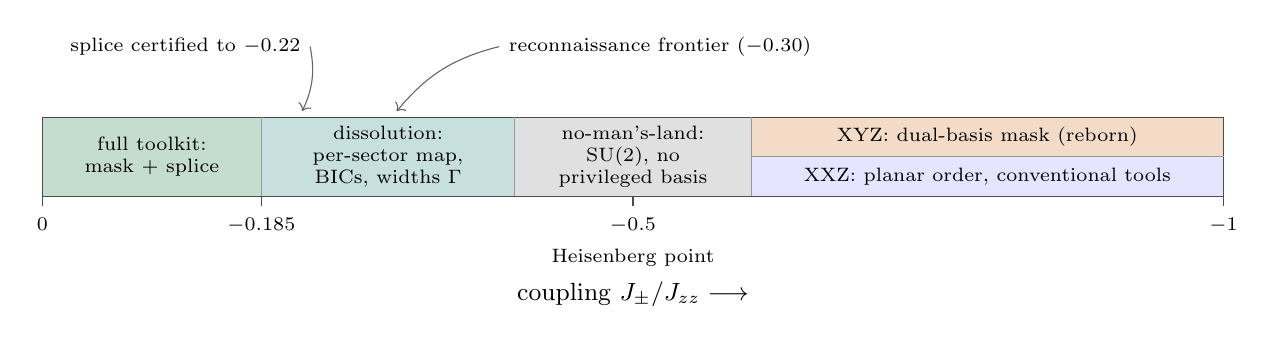
\begin{tikzpicture}
% bar: x = 15*|Jpm/Jzz|
\fill[goodcol!25] (0,0) rectangle (2.78,1);
\fill[icecol!22] (2.78,0) rectangle (6.0,1);
\fill[black!12] (6.0,0) rectangle (9.0,1);
\fill[spincol!22] (9.0,0.5) rectangle (15,1);
\fill[blue!10] (9.0,0) rectangle (15,0.5);
\draw[black!70] (0,0) rectangle (15,1);
\draw[black!40] (2.78,0) -- (2.78,1);
\draw[black!40] (6.0,0) -- (6.0,1);
\draw[black!40] (9.0,0) -- (9.0,1);
\draw[black!40] (9.0,0.5) -- (15,0.5);
% region labels
\node[font=\scriptsize,align=center] at (1.39,0.5) {full toolkit:\\ mask $+$ splice};
\node[font=\scriptsize,align=center] at (4.39,0.5) {dissolution:\\ per-sector map,\\ BICs, widths $\Gamma$};
\node[font=\scriptsize,align=center] at (7.5,0.5) {no-man's-land:\\ SU(2), no\\ privileged basis};
\node[font=\scriptsize,align=center] at (12.0,0.75) {XYZ: dual-basis mask (reborn)};
\node[font=\scriptsize,align=center] at (12.0,0.25) {XXZ: planar order, conventional tools};
% ticks
\foreach \x/\l in {0/$0$, 2.78/$-0.185$, 7.5/$-0.5$, 15/$-1$}{
  \draw[black!70] (\x,0) -- (\x,-0.12);
  \node[font=\scriptsize,below] at (\x,-0.15) {\l};
}
\node[font=\scriptsize,below] at (7.5,-0.55) {Heisenberg point};
% annotations above
\node[font=\scriptsize,left] at (3.4,1.9) {splice certified to $-0.22$};
\draw[->,black!60] (3.4,1.9) to[bend left=18] (3.3,1.08);
\node[font=\scriptsize,right] at (5.8,1.9) {reconnaissance frontier ($-0.30$)};
\draw[->,black!60] (5.8,1.9) to[bend right=18] (4.5,1.08);
\node[font=\small] at (7.5,-1.25) {coupling $\Jpm/\Jzz \longrightarrow$};
\end{tikzpicture}
\caption{The regime map, with instrument handoffs.  Green: weak coupling,
where mask, counterterm, and splice all operate.  Teal: the dissolution
regime, where band physics belongs to the per-sector masked map (BICs and
Gamow widths) and $H+C$ survives only as an estimate with quoted residue.
Grey: the shell around the Heisenberg point, where SU(2) symmetry makes
every ice basis a convention and no topological cleaning is meaningful.
Beyond: in XYZ materials the whole machinery is reborn in the dominant
axis's basis (orange); in strict XXZ the planar magnet takes over and
conventional finite-size tools --- including honest twist averaging ---
are the right ones (blue).  Boundaries drawn at the 16-site values; their
precise location is itself a finite-size quantity.}
\label{fig:regimemap}
\end{figure}

%=====================================================================
\section{Wrong turns, kept on purpose}
\label{sec:wrongturns}

Science reporting usually deletes the dead ends.  This campaign keeps them,
because each one carries a transferable rule.

\begin{center}
\small
\begin{tabular}{p{5.6cm}p{8.6cm}}
\toprule
\textbf{The wrong turn} & \textbf{The rule it taught}\\
\midrule
``Twist averaging removes winding contamination'' (original claim, retracted)
& Phases attach to virtual routes, not loop topology.  Compute the object you
claim vanishes.\\[2pt]
The twist period was taken as $2\pi$; corrected to $4\pi$
& The transport quantum is \emph{half} a box vector
(Eq.~\ref{eq:rho}); flux periods follow from the charge actually
transported, not from habit.\\[2pt]
``The label is emergent electric charge''
& The ice manifold is charge-free; the label is the \emph{magnetization
displacement}.  Same machinery, correct words --- and the words matter when
you predict what couples to it.\\[2pt]
A spectral counting theorem was applied to the masked map, yielding 31\,233
``levels'' in a 12\,870-state space
& The theorem's hypotheses (it applies to genuine sub-blocks of a Hermitian
matrix) failed for the masked object.  Check hypotheses \emph{before}
trusting a theorem's output; a nonsense count was the only warning.\\[2pt]
The ``anchoring residue'' peak (a week of theory built on it)
& It was an unconverged solver ($3$ fixed-point rounds at convergence rate
$\sim0.5$).  Converge to $10^{-12}$ before interpreting $10^{-2}$.\\[2pt]
Sector symmetrisation; catalogue counterterms
& Corrections must be derived from the exact object, not from a plausible
model of it; both ``improvements'' made things worse.\\[2pt]
Sparse eigensolver used to count degenerate levels
& It silently returned 4 of 7 copies of a degenerate level.  Never use a
lone sparse solve as a multiplicity referee.\\[2pt]
Peak positions read off a 3000-point grid ``agreed to 0.00\%''
& The grid step was 0.585\%; the agreement was quantization, not accuracy.
Refine and interpolate before quoting exponents.\\
\bottomrule
\end{tabular}
\end{center}

%=====================================================================
\section{Cast of characters}

\begin{center}
\small
\begin{tabular}{lp{10.6cm}}
\toprule
symbol / term & meaning\\
\midrule
$\Jzz$ & the ice-rule interaction; the unit of energy; spinon cost scale\\
$\Jpm$ & the quantum (flip) interaction; the one dial; negative for cerium
pyrochlores\\
ice manifold & all spin patterns obeying two-in--two-out on every
tetrahedron (90 states on 16 sites, 2970 on 32)\\
spinon & a tetrahedron violating the ice rule; the emergent electric charge;
energy $\sim\Jzz$\\
ring exchange & collective flip of a closed loop of spins that stays inside
the ice manifold\\
$\gsix=12|\Jpm|^3/\Jzz^2$ & strength of the hexagon ring exchange = the
photon scale = the real physics\\
$\gfour=4\Jpm^2/\Jzz$ & strength of the wrap-around four-site loop = the
box artifact\\
winding $w$ & how many times a loop wraps each glued direction; the complete
topological label\\
transport $\rho$ & magnetization displacement of a flip process;
$\rho=\frac12 w\cdot L$ exactly\\
sector & family of ice states sharing one polarization value; 25 on 16
sites, 85 on 32\\
the mask & deletion of every amplitude connecting different sectors
= exact removal of all winding processes\\
$F(z)$ & the Feshbach map: the ice-block amplitude table with all spinon
excursions folded in exactly, at asking-energy $z$\\
$Z$, ice weight & the fraction of an exact eigenstate living inside the
ice manifold, $Z_n=\langle n|P|n\rangle=\|P|n\rangle\|^2\in[0,1]$ (also
called the residue or purity); $1-Z$ = spinon dressing = the error and
convergence rate of everything approximate; sum rule
$\sum_n Z_n=\mathrm{Tr}\,P=90$ over the whole spectrum\\
$H+C$ & full-space Hamiltonian with the artifact counterterm; whole
spectrum at once; residue grows as $1-Z$\\
the splice & $H+C$ spectrum with its lowest 90 levels replaced by the exact
masked roots; best of both\\
BIC & bound state in the continuum: a winding-free level above the
continuum edge, forbidden to decay by transport symmetry\\
girth engineering & choosing the cell shape to maximize the shortest
wrap-around loop, demoting the irreducible artifact\\
twist $\theta$ & phase on flips crossing the glued edge; useless for
topology (Sec.~\ref{sec:twist}), essential for densifying the spinon
continuum (Sec.~\ref{sec:roadahead})\\
Gamow root & complex self-consistent energy $E-i\Gamma/2$, appearing when a
level meets its \emph{own} sector's continuum; $\Gamma$ is a physical
lifetime, not an error\\
mirror map $G(z)$ & the Feshbach fold run the other way: ice space folded
into the spinon block; cheap because $PHP$ is diagonal\\
truncation level $L$ & keep spinon states within $L$ pair-flip moves of
the ice manifold: the depth of virtual excursion followed; the $L$-ladder
drift is the large-cluster error bar\\
bordered matrix $M_s$ & sector ice block bordered by the (truncated)
spinon space; Hermitian, so sector spectra come from sparse Lanczos with
no anchor --- the calibrated crossing instrument\\
two-sided fold & counterterm-free thermodynamics: remove the 90
highest-$Z_n$ raw levels (wherever they sit), insert the masked roots at
weight one; the mirror map supplies $Z_n$ as the \emph{identifier} --- the
weighted version fails (hijacked ensemble)\\
$Z$-rank gap & jump in ice weight between the last removed and first kept
raw level; bimodal at weak coupling, closes by $-0.20$ --- the continuous
dial of band identity, and the obstruction theorem seen in data\\
third peak & the low-$T$ $C(T)$ structure below the ring anomaly; three
distinct causes --- counterterm splitting (fake), internal band gap
(real), ground-multiplicity change (real) --- see
Sec.~\ref{sec:thirdpeak}\\
Heisenberg point & $\Jpm=-\Jzz/2$: full SU(2) symmetry; every ice basis
becomes a convention and the mask becomes axis-dependent --- the method's
structural boundary\\
axis spread & disagreement between masked results built on the $z$, $x$,
$y$ bases; measures how much meaning the mask retains as the Heisenberg
point approaches\\
axis-permutation duality & exact XYZ relabeling of local axes; transfers
the entire machinery to whichever coupling dominates\\
\bottomrule
\end{tabular}
\end{center}

\vspace{1em}
\begin{plainwords}
The campaign in four sentences.  A small glued simulation box invents a
wrap-around quantum process that is stronger than the real photon physics of
quantum spin ice, and the popular twist-averaging remedy provably cannot
remove it.  Measuring how far each process transports magnetization
identifies the wrap-arounds exactly, and deleting them (the mask) is a
provably maximal, provably safe cleaning that works at any coupling once
combined with the Feshbach fold.  With the artifact gone, the true photon
scale, its flux law, its non-decay, and a previously hidden physical anomaly
all emerge --- and the remaining error is the box itself.  The next campaign
attacks that error on three independent fronts: the mask for topology,
cell-shape optimization for the irreducible wrap-pairs, and twist averaging
--- reborn in its legitimate role --- to give the virtual spinons a dense
continuum to live in.  The method's writ runs from weak coupling all the
way to the Heisenberg point, where SU(2) symmetry turns the description
itself into a convention --- and past it, in the XYZ models of the real
materials, everything is reborn in the basis of the new dominant axis.
\end{plainwords}

\end{document}
